\documentclass[aspectratio=1610,francais,envcountsect]{beamer}
\usepackage[linesnumbered,vlined]{algorithm2e}
\usepackage[french]{babel}
\usepackage{graphicx}
\usepackage[T1]{fontenc}
\usepackage[utf8]{inputenc}
\usepackage{etex}
% \usepackage[zerostyle=d]{newtxtt}

\newtheorem{property}[theorem]{Propriété}
\usepackage{amsmath}
\DeclareMathOperator*{\argmax}{arg\,max}

\renewcommand{\sfdefault}{cmbr}
\usefonttheme[onlymath]{serif}
\usepackage{pifont}
%\usepackage[scaled=1,lining]{FiraSans}
\usepackage{inconsolata}
\setbeamertemplate{theorems}[numbered]
\setbeamertemplate{frametitle continuation}[from second][\insertcontinuationtext]

\newcommand{\mainstyle}{
  \setbeamertemplate{footline}{
    \hbox{%
      \begin{beamercolorbox}[wd=.2\paperwidth,ht=2ex,dp=1ex,left]{author in head/foot}%
        \hspace*{1em}\usebeamerfont{author in head/foot}\insertshortauthor
      \end{beamercolorbox}%
      \begin{beamercolorbox}[wd=.6\paperwidth,ht=2ex,dp=1ex,center]{title in head/foot}%
        \usebeamerfont{title in head/foot}\insertshorttitle
      \end{beamercolorbox}%
      \begin{beamercolorbox}[wd=.2\paperwidth,ht=2ex,dp=1ex,right]{page number in head/foot}%
        \usebeamerfont{page number in head/foot}\insertframenumber{}% /\insertpresentationendframe
        \kern1em 
      \end{beamercolorbox}
    }
  }
  \setbeamercolor{section in head/foot}{bg=black,fg=white}
  %\setbeamercolor{subsection in head/foot}{bg=black,fg=white}
}

\mode
<beamer>
{\usenavigationsymbolstemplate{}
}

\usepackage{tikz}
\usetikzlibrary{trees,positioning,fit,arrows}

\title{Paradigmes algorithmiques}
\subtitle{Quelques méthodes de conception d'algorithmes}

\author[Gauthier Picard]{Gauthier Picard \and (Roland Jégou)}

\date{MINES Saint-Étienne}

\mainstyle{}


\begin{document}

\setbeamertemplate{headline}{}

{ \setbeamertemplate{headline}{} \setbeamertemplate{footline}{}
  \maketitle
}

\section*{Introduction}

\begin{frame}[allowframebreaks]
  \frametitle{Introduction} Le processus général de résolution
  algorithmique (ou informatique) d'un problème peut grossièrement se
  décomposer en trois phases :

  \begin{center}
    LE PROBLÈME $\to$ L'ALGORITHME $\to$ LE PROGRAMME
  \end{center}

  \bigskip

  \begin{center}
    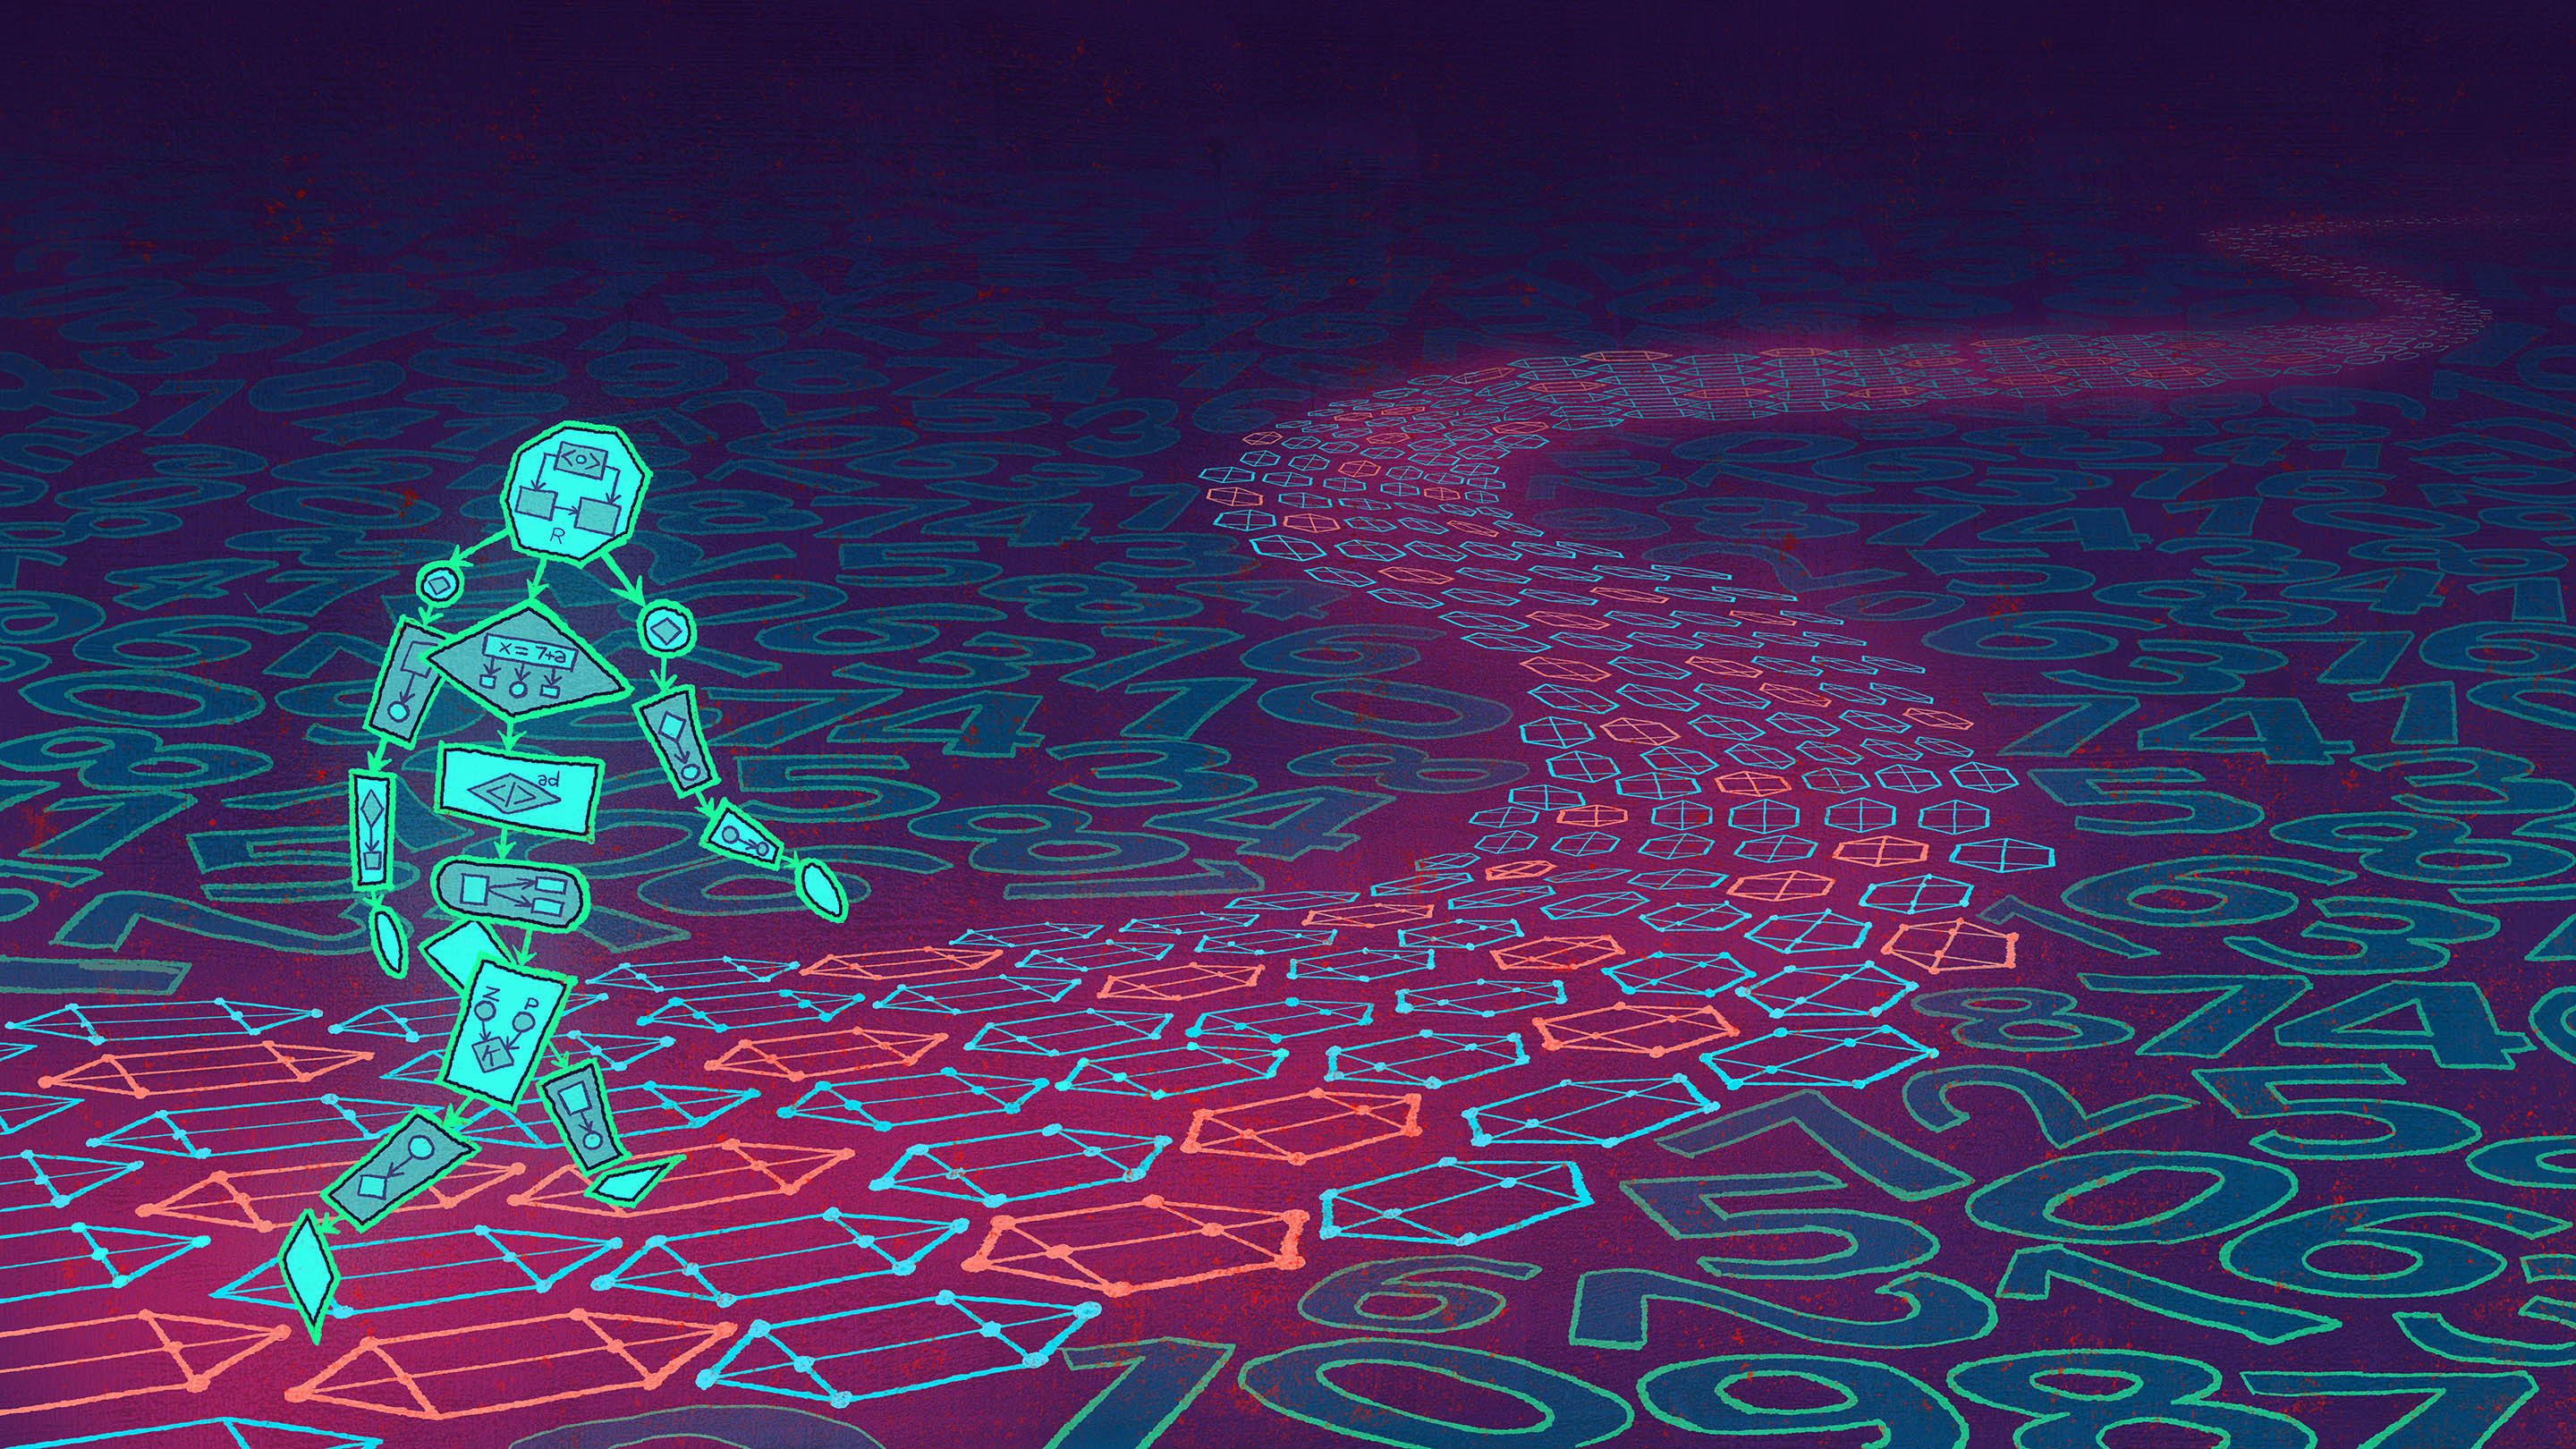
\includegraphics[height=4cm]{algorithm.jpg}
  \end{center}

  \framebreak

  \begin{block}{Le problème}
    \begin{itemize}
    \item Préciser les \structure{spécifications} : données ?
      résultats ?  environnement ?
    \item \structure{Modélisation} : structures mathématiques ?
      propriétés ? problème déjà connu, ... ?
    \item \structure{Modularisation} : décomposition en sous
      problèmes, sous problèmes plus simples, indépendants, ... ?
    \end{itemize}
  \end{block}

  \framebreak

  \begin{block}{L'algorithme}
    \begin{itemize}
    \item \structure{Conception} : méthodes de conception
      d'algorithmes ?
    \item \structure{Écriture} dans un pseudo langage ?
    \item \structure{Structures de données} ?
    \item \structure{Analyse} : preuve (fin, validité), efficacité
      (complexités) ?
    \end{itemize}
  \end{block}

  \framebreak

  \begin{block}{Le programme}
    \begin{itemize}
    \item \structure{Traduction} de l'algorithme dans un langage de
      programmation précis dans un environnement précis ?
    \item \structure{Mise au point} : tests ?  documentation ? ...
    \end{itemize}
  \end{block}

  \framebreak

  \begin{exampleblock}{En pratique}
    \begin{itemize}
    \item nombreux allers-retours entre ces étapes
    \item minimiser par une conception descendante
    \item du général au particulier, par l'utilisation de la
      modularisation
    
      \begin{itemize}
      \item e.g. division en sous problèmes bien spécifiés et dont les
        dépendances doivent être clairement mises en évidence (sorte
        de graphe de précédence des différents «~morceaux~» : sous
        problèmes, modules, sous programmes, fonctions, ...)
      \end{itemize}
    \end{itemize}
  \end{exampleblock}

\end{frame}

\begin{frame}[allowframebreaks]
  \frametitle{Questions d'algorithmique}

  \begin{block}{Outils de modélisations ?}
    \begin{itemize}
    \item De nombreuses \structure{structures mathématiques} sont très
      utiles (domaine des mathématiques discrètes, de la combinatoire)
      :
      \begin{itemize}
      \item ensembles « particuliers » (suites, piles, files,
        tableaux, matrices, ...)
      \item arborescences (structures fondamentales en informatique)
      \item graphes (orientés ou non)
      \item multigraphes
      \item ensembles ordonnés
      \item hypergraphes
      \item ...
      \end{itemize}
    \item Nécessité de \structure{connaître ces « objets »}, leurs
      propriétés et leurs mises en œuvre
    \end{itemize}

  \end{block}

  \framebreak

  \begin{block}{Conception d'algorithmes ?}
    \begin{itemize}
    \item \structure{Pas de recette miracle} mais quelques méthodes
      générales de résolution
    \item Elles ne fonctionnent pas toujours mais elles ont le mérite
      de donner des pistes et de souvent fournir une solution
    \item On parle de \structure{Paradigmes Algorithmiques}
    \end{itemize}
  \end{block}

  \framebreak

  \begin{block}{Comparaison d'algorithmes ?}
    \begin{itemize}
    \item Outil privilégié = \structure{Complexité} (en fait
      \emph{les} complexités, voir suite)
      \begin{itemize}
      \item Donne une mesure objective de \structure{l'efficacité}
        d'un algorithme
      \end{itemize}
    \item Nécessité de maîtriser les calculs de complexités et de
      connaître certains résultats
    \end{itemize}
  \end{block}

  \framebreak

  \begin{block}{Trouver de meilleurs algorithmes ?}
    \begin{itemize}
    \item Essai de \structure{plusieurs stratégie}s algorithmiques et
      de différentes structures de données
    \item Comment déterminer la \structure{difficulté intrinsèque}
      d'un problème ?
    \item Calculs de \structure{bornes inférieures} ?
    \item Algorithmes optimaux ?
    \item \structure{Problèmes difficiles} : Théorie de la Complexité
      (classes P, NP ; NP-complétude ; NP-difficulté ...)
    \end{itemize}

  \end{block}
\end{frame}

\begin{frame}[allowframebreaks]
  \frametitle{Contenu de ce cours}

  \begin{block}{Recherche Exhaustive}
    Elle consiste à examiner directement ou indirectement l'ensemble
    de toutes les solutions possibles (solutions admissibles ou
    réalisables)
  \end{block}

\begin{block}{Divide-and-Conquer, Récursivité}
  On résout le problème, en général récursivement, en le décomposant
  en sous problèmes de même nature, et en « fusionnant » les sous
  solutions obtenues
\end{block}

\begin{block}{Prétraitement}
  Il s'agit ici d'organiser, de structurer des données pour mieux
  résoudre le problème
\end{block}

\begin{block}{Méthodes incrémentales}
  Ces méthodes construisent la solution en considérant les éléments de
  la donnée les uns après les autres
\end{block}

\begin{block}{Transformation, Réduction}
  L'idée est de ramener le problème à résoudre à un autre problème
  déjà connu. Cela permet aussi d'établir des résultats sur des bornes
  inférieures
\end{block}

\begin{block}{Programmation Dynamique}
  Le problème initial est décomposé en sous problèmes qui sont résolus
  de façon incrémentales, et non récursives, par tailles croissantes
\end{block}

\begin{block}{Algorithmes Gloutons}
  Le problème est résolu de façon incrémentale en faisant à chaque
  étape un choix local qui n'est jamais remis en question
\end{block}

% \begin{block}{Parcours de Graphes}
%   La notion de graphe est un outil de modélisation de très nombreux
%   problèmes, voir Cours de Recherche Opérationnelle par
%   exemple. Leurs manipulations nécessitent des techniques
%   particulières, souvent à base de parcours
% \end{block}

% \begin{block}{Méthodes Approximatives}
%   Ces méthodes, donnant une solution approchée à un problème, sont
%   utilisées pour les problèmes difficiles. Elles doivent être
%   rapides (polynomiales) et donner une solution réalisable qu'on
%   espère proche de l'optimal
% \end{block}

\end{frame}


\begin{frame}
  \frametitle{Menu}
  \tableofcontents[hidesubsections]
\end{frame}
  
\AtBeginSection[] { \setcounter{tocdepth}{2} \frame<handout:0> {
    \frametitle{Menu}
    \tableofcontents[current,currentsubsection,hidesubsections]
  } }

\section{Recherche exhaustive}

\begin{frame}
  \frametitle{Recherche exhaustive}

  Appellée aussi \structure{Méthode Naïve} (ou Algorithme Naïf)\\en
  anglais «~\emph{Brute Force Method}~», «~\emph{Naive Algorithm}~»

  \bigskip
  
  \begin{alertblock}{Principe}
    \emph{Examiner tous les cas possibles}
  \end{alertblock}

  \bigskip
  
  \begin{itemize}
  \item Quoi de plus simple ?
  \item Encore faut-il qu'il y ait un \structure{nombre fini de cas
      possibles} (toujours vrai ici)
  \item Dans ce cas, cette méthode donne toujours une solution en
    \structure{temps polynomial ou exponentiel} (suivant le nombre de
    cas, d'où l'intérêt de savoir « compter »)
  \item Mais c'est une méthode pas toujours facile à mettre en œuvre
    (i.e. programmer)
  \end{itemize}

  C'est la méthode de base de résolution des \structure{Problèmes
    d'Optimisation Combinatoire} (POC), car à la base des
  \structure{Méthodes Arborescentes} (e.g. \emph{branch-and-bound})

\end{frame}

\begin{frame}[allowframebreaks]
  \frametitle{Problèmes d'optimisation combinatoire}

  \begin{definition}[POC]%{Problème d'optimisation combinatoire}
    \begin{description}
    \item[Donnée] $S$ ensemble fini et $f$ une fonction de $S$ vers
      les entiers, $f : S \to \mathbb{N}$
    \item[Question] On cherche $s_0 \in S$ telle que
      $f(s_0) = opt \{ f(s), s\in S\}$ où $opt$ signifie $min$ ou
      $max$
    \end{description}
  \end{definition}

  Autrement dit, on cherche dans un ensemble fini $S$ (ensemble des
  \structure{Solutions Réalisables ou Admissibles}) un élément $s_0$
  optimisant une certaine fonction $f$ dite \structure{Fonction
    Objectif ou Economique}

  \framebreak

  Souvent il existe un ensemble fini $E$ sous-jacent et une fonction
  $c$ associant un coût (profit, distance, poids, profit, capacité,
  ...) à tout élément de $E$ tels que :

  \begin{itemize}
  \item $S \subseteq \mathfrak{P}(E)$ ($S$ = famille de parties de
    $E$)\\ i.e.
    $S = \{ s \subseteq E, s \text{ vérifie une certaine propriété }
    \pi \}$
  \item $f(s)= \sum_{e\in S} c(e), \forall s \in S$
  \end{itemize}

  Le problème est alors dit \structure{Problème d'Optimisation
    Combinatoire à Fonction Objectif Séparée} (POC-FOS)
  
\end{frame}

\begin{frame}
  \frametitle{Propriétés de ces ensembles}

  On note $\mathfrak{P}(E)$ l'ensemble des parties de $E$ et
  $\mathfrak{P}_k(E)$ l'ensemble des parties de $E$ ayant $k$ éléments
  ($0 \leq k \leq n$)
  
  \begin{equation}
    |\mathfrak{P}(E)|=2^n\label{eq:1}
  \end{equation}
  
  \begin{equation}
    |\mathfrak{P}(E)| = C^k_n = \binom{k}{n} = \frac{n!}{k!(n - k )!} \in \theta(n^k)  \label{eq:2}
  \end{equation}

  Le nombre de suites ordonnées de $k$ éléments de distincts de $E$
  (arrangements) est

\begin{equation}
  A_n^k =n \times (n - 1) \times \ldots  \times (n - k+1) = \frac{n!}{(n - k)!}
\end{equation}

\bigskip

Si $F$ est un ensemble ayant $m$ éléments, alors le nombre
d'applications de $E$ dans $F$ est égal à $m^n$ (l'ensemble $A(E, F)$
des applications de $E$ dans $F$ est aussi noté $F^E$)
\end{frame}

\begin{frame}
  \frametitle{Génération exhaustive}
  \begin{itemize}
  \item Ainsi pour un POC-FOS il est toujours possible de résoudre le
    problème par \structure{Génération Exhaustive} = génération
    arborescente de tous les cas possibles : il y a en effet $2^n$
    solutions potentielles à générer, quand $E$ a $n$ éléments
  
  
  \item On peut en effet associer à chaque élément $i$ une variable
    booléenne $x_i$, valant $1$ si l'élément $i$ est choisi et $0$
    sinon

    % Un petit exercice : comment peut-on effectivement mettre en
    % œuvre une telle méthode ?
  
  
  \item Mais, même si elle est efficace quand $n$ est petit, cela
    s'avère vite irréaliste par rapport aux temps de calcul, lorsque
    les tailles des données à traiter sont grandes
  \end{itemize}
  \begin{example}
    Si $n = 100$, quelle serait la durée de la méthode sur une machine
    pouvant examiner chaque solution potentielle en $10^{-9}$ seconde
    ?

    \pause

    \begin{itemize}
    \item $2^{100} \approx 1.25 \times 10^{30}$ solutions
    \item Temps =
      $1.26 \times 10^{30} \times 10^{-9} \approx 1.26 \times 10^{21}$
      secondes $\approx 2.11\times10^{19}$ minutes
      $\approx 3.52\times10^{17}$ heures $\approx 1.46\times10^{16}$
      jours $\approx 4 \times 10^{13}$ ans
    \end{itemize}

  \end{example}

\end{frame}

\begin{frame}[allowframebreaks]
  \frametitle{Exemples de problèmes}

  \begin{definition}[Paire de Points la Plus Proche (P$^\mathsf{4}$)]

    \begin{description}
    \item[Données] Soit $E = \{p_1, p_2, \ldots , p_n\}$ un ensemble
      de $n$ points du plan, chacun étant donné par ses coordonnées
      $p_i = (x_i, y_i)$
    \item[Question] Trouver dans $E$ deux points dont la distance est
      minimale
    \end{description}
  \end{definition}

  \begin{center}
    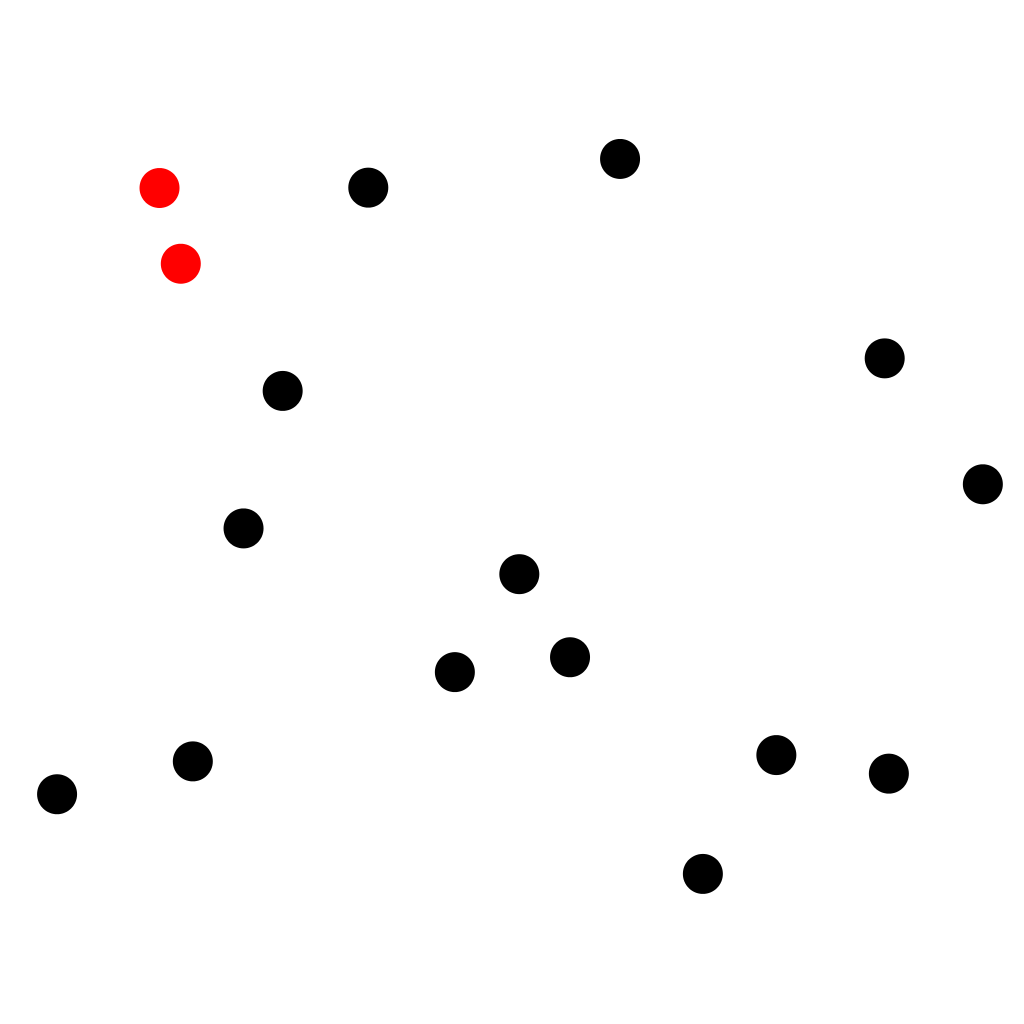
\includegraphics[height=4cm]{p4.png}
  \end{center}


  \framebreak

  \begin{definition}[Arbre Recouvrant Minimal (ou Minimal Spanning
    Tree)]

    \begin{description}
    \item[Données] Soit $G = (X, E, d)$ un graphe simple non orienté
      valué où $d$ est une fonction qui attribue une valeur à chacune
      des arêtes (distance, coût, capacité, temps, \ldots)
    \item [Question] Construire un arbre recouvrant $T = (X, E)$ de
      $G$ qui soit de coût (somme des valeurs des arêtes) minimal
    \end{description}
  \end{definition}

  \begin{columns}
    \begin{column}{0.5\columnwidth}
      \begin{theorem}[Cayley, 1897]
        Il existe $n^{n - 2}$ arbres ayant pour sommets $n$ points
        distincts du plan (ou pour le graphe complet $K_n$)
      \end{theorem}
    \end{column}

    \begin{column}{0.5\columnwidth}
      \begin{center}
        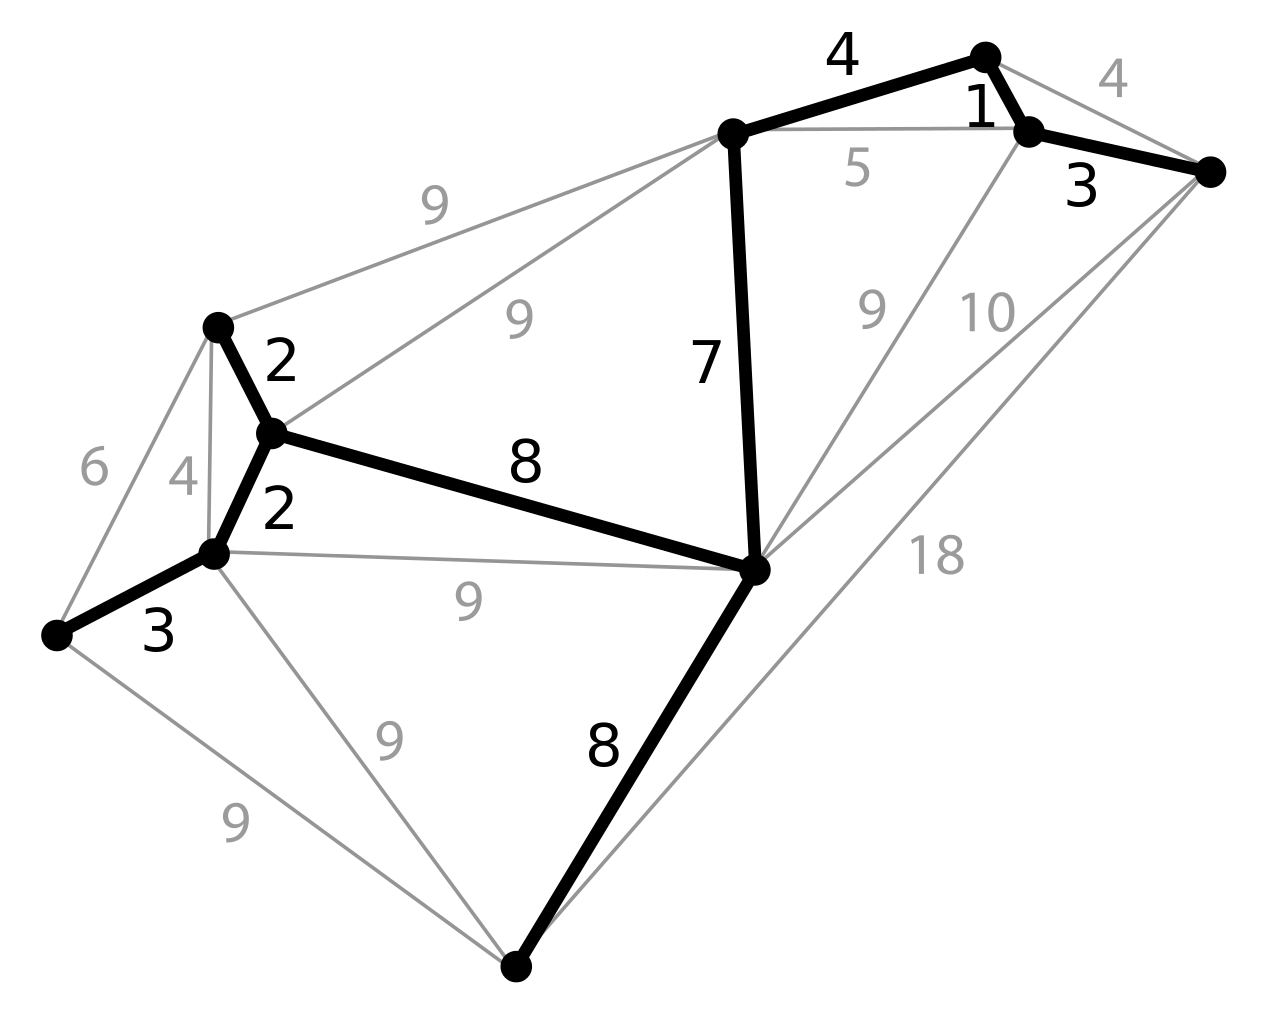
\includegraphics[width=0.7\columnwidth]{spanning.png}
      \end{center}
    \end{column}
  \end{columns}


  \framebreak

  \begin{definition}[Enveloppe Convexe de $n$ points du plan (EC)]

    \begin{description}
    \item [Données] Soit $E = \{p_1, p_2,\ldots , p_n\}$ un ensemble
      de $n$ points du plan, chacun étant donné par ses coordonnées
      $p_i = (x_i, y_i)$

    \item[Question] Déterminer l’Enveloppe Convexe de $E$, $EC(E)$,
      c’est-à-dire le plus petit ensemble convexe du plan contenant
      $E$
    \end{description}
  \end{definition}

  \begin{center}
    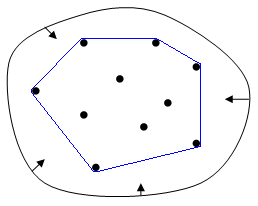
\includegraphics[width=0.3\columnwidth]{hull.png}
  \end{center}

  \framebreak

  \begin{definition}[Voyageur de Commerce (PVC)]

    \begin{description}
    \item [Données] $G = (X, U, d)$ un graphe orienté valué où $d$
      attribue à chaque arc $u$ une valuation $d(u)$ (coût, distance,
      temps, \ldots)
    \item [Question] Déterminer un circuit hamiltonien de $G$ de
      longueur minimale
    \end{description}
  \end{definition}

  \begin{columns}
    \begin{column}{0.5\columnwidth}
      \begin{theorem}
        Il y a $1/2 \times (n - 1)!$ cycles possibles dans un graphe
        dans le plan
      \end{theorem}
    \end{column}

    \begin{column}{0.5\columnwidth}
      \begin{center}
        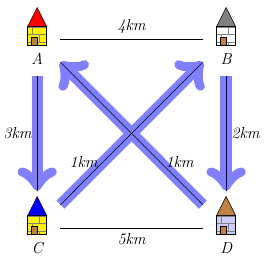
\includegraphics[width=0.7\columnwidth]{tsp.png}
      \end{center}
    \end{column}
  \end{columns}


  \framebreak

  \begin{definition}[Problème du Sac à Dos (SAD)]

    \begin{description}
    \item [Données] $n$ objets, numérotés $1, 2, \ldots, n$ et
      d’utilités et poids respectifs $u_1, u_2, \ldots , u_n$ et
      $p_1, p_2, \ldots , p_n$ (entiers positifs) et d’un sac à dos de
      poids maximal $P$
    \item [Question] Comment remplir le sac en prenant au plus un
      exemplaire de chaque objet et sans dépasser le poids maximal $P$
      pour maximiser son utilité ?
    \end{description}
  \end{definition}

  \begin{center}
    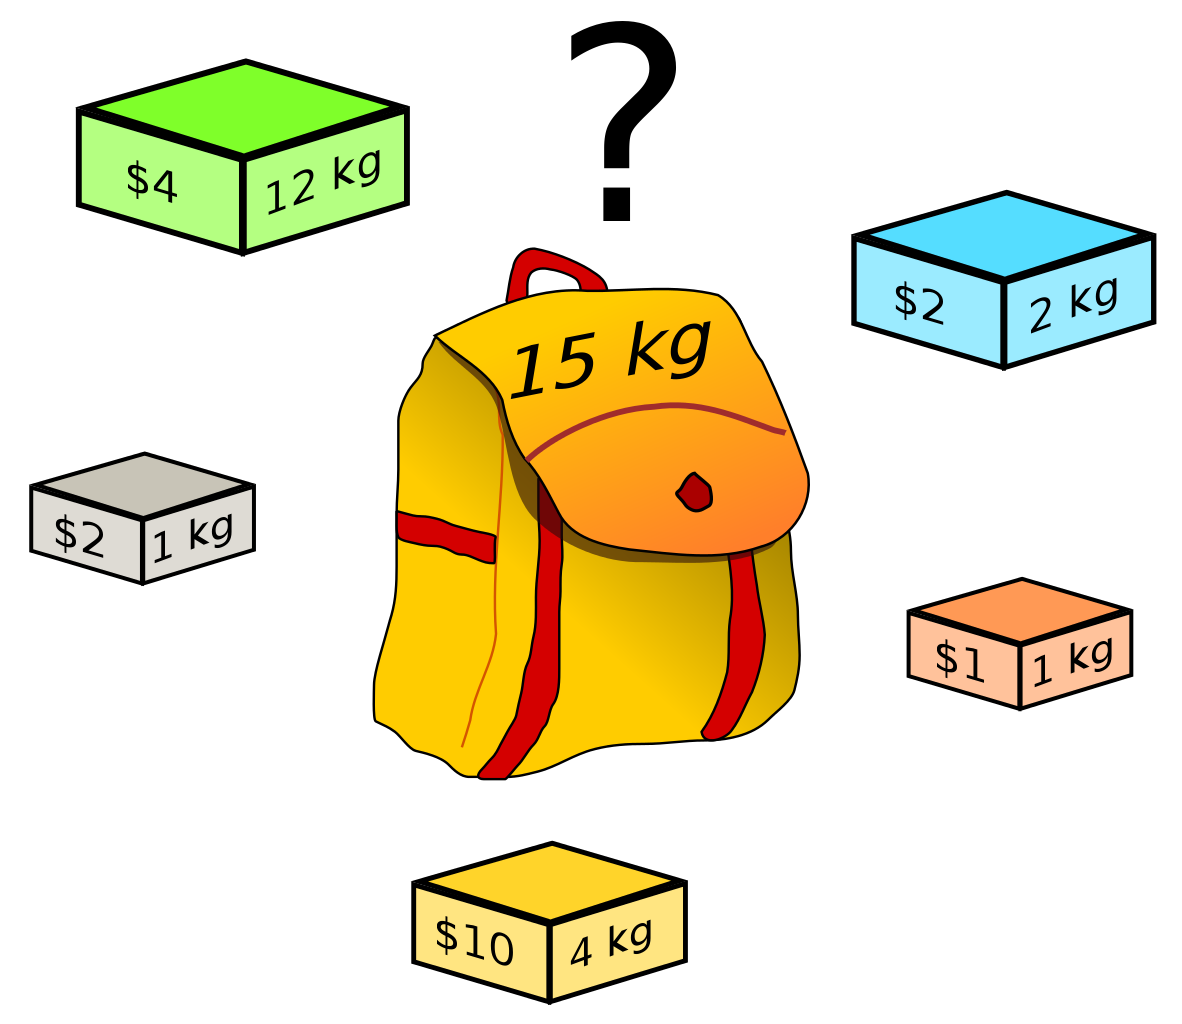
\includegraphics[width=0.3\columnwidth]{knapsack.png}
  \end{center}

  \framebreak

  \begin{definition}[Problème de la Somme (SOM)]

    \begin{description}
    \item [Données] Soit $V = \{ v_1, v_2, \ldots , v_n\}$ un ensemble
      d’entiers strictement positifs (valeurs, poids, durées, \ldots)
      et $S$ un entier, avec $v_1 \leq v_2 \leq \ldots \leq v_n$
    \item [Question] Existe-t-il un sous-ensemble $W$ de $V$ dont la
      somme des éléments est égale à $S$ ou s’en approche de façon
      optimale ?
    \end{description}
  \end{definition}

  \framebreak

  \begin{definition}[Le Problème du Tri (TRI)]
    \begin{description}
    \item [Données] Soit $E = \{e_1, e_2,\ldots , e_n\}$ un ensemble
      de $n$ éléments muni d’un ordre total « $\leq$ », c’est-à-dire
      $\forall i, j$ on a soit $e_i \leq e_j$ soit $e_j \leq e_i$
    \item [Question] Ordonner totalement les éléments de $E$
    \end{description}

  \end{definition}


  \begin{center}
    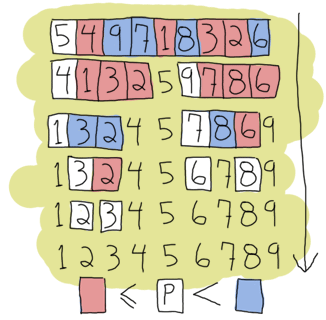
\includegraphics[width=0.3\columnwidth]{quicksort.png}
  \end{center}

\end{frame}

\begin{frame}[allowframebreaks]
  \frametitle{Méthode Branch-and-Bound}

  La méthode SEP (\structure{Séparation et Evaluation Progressive} ou
  \structure{\emph{Branch-and-Bound}}, ou BB) est basée sur la
  Recherche Exhaustive mais permet d'atténuer l'explosion combinatoire
  \bigskip
  
  \begin{alertblock}{Principe}
    \it Parcourir implicitement et de façon arborescente
    (\structure{séparation}), l'ensemble des solutions potentielles en
    tirant parti :
  
    \begin{itemize}
    \item d'un ordre de sélection des variables
    \item d'une compatibilité des variables (le choix d'une variable
      peut éliminer ou au contraire impliquer d'autres variables)
    \item du calcul d'une fonction à chaque étape (représentant une
      borne inférieure pour un problème de minimisation ou un borne
      supérieure pour un problème de maximisation) permettant
      d'orienter la recherche et d'éliminer des recherches
      infructueuses (\structure{évaluation})
    \end{itemize}
  \end{alertblock}
  \framebreak

  \begin{block}{Borne inférieure}
    \begin{itemize}
    \item Pour un problème de \structure{Maximisation} il faut
      calculer une Borne Supérieure, $BS(x)$, en chaque sommet $x$ de
      l' arborescence de l' exploration telle que toutes les solutions
      de la sous arborescence correspondante, $A(x)$, seront au plus
      égales à $BS(x)$
  
  
    \item Si $BS(x)$ est inférieure à un maximum déjà trouvé alors il
      est inutile d'explorer $A(x)$
    \end{itemize}

  \end{block}


  \begin{block}{Borne supérieure}
    \begin{itemize}
    \item Pour un problème de \structure{Minimisation} il faut
      calculer une Borne Inférieure, $BI(x)$, en chaque sommet $x$ de
      l'arborescence de l'exploration telle que toutes les solutions
      de la sous arborescence correspondante, $A(x)$, seront au moins
      égales à $BI(x)$
  
    \item Si $BI(x)$ est supérieure à un minimum déjà trouvé alors il
      est inutile d'explorer $A(x)$
    \end{itemize}

  \end{block}

  Dans les deux cas, la recherche reprend au\structure{ sommet le plus
    prometteur} c'est-à-dire où la borne, $BS(x)$ ou $BI(x)$, est la
  meilleure, soit la plus grande pour un problème de Maximisation soit
  un le plus petite pour un problème de Minimisation
\end{frame}

\begin{frame}[fragile]
  \frametitle{Branch-and-Bound} \framesubtitle{Représentation
    algorithmique}
  \begin{algorithm}[H]
    \small \DontPrintSemicolon \SetKwProg{Fn}{Function}{}{}
    \SetKwFunction{BandB}{branch\_and\_bound}
    \SetKwFunction{isTrivial}{is\_trivial}
    \SetKwFunction{trivialSolve}{trivial\_solve}
    \SetKwFunction{branch}{branch} pb $\leftarrow$ \texttt{null}\;
    best $\leftarrow$ $+\infty$\; \Fn{\BandB{pb$_0$}}{
      \eIf{\isTrivial{$pb_0$}}{ local $\leftarrow$
        \trivialSolve{pb$_0$}\; \If{local < best}{ best $\leftarrow$
          local\; pb $\leftarrow$ pb$_0$ } }{ local $\leftarrow$
        $BI($pb$_0)$\; \If{local < best}{ (pb$_1$, pb$_2$)
          $\leftarrow$ \branch{pb$_0$}\; \BandB{$pb_1$}\;
          \BandB{$pb_2$}\; } } }
  \end{algorithm}

  
\end{frame}

\begin{frame}
  \frametitle{Exemple d'utilisation de Branch-and-Bound}
  \framesubtitle{SAD}

  \begin{example}[SAD]
    Comment remplir au mieux un sac de quantité max $P = 10$ avec les
    objets suivants :

    \begin{center}
      \begin{tabular}{l|lllll}
        &A&B&C&D&E\\
        \hline
        $p_i$&2&3.14&1.98&5&3\\
        $u_i$&40&50&100&95&30
      \end{tabular}
    \end{center}

  \end{example}
\end{frame}

\begin{frame}
  \frametitle{Exemple d'utilisation de Branch-and-Bound}
  \framesubtitle{SAD}

  \begin{example}[Résolution exhaustive]
    \bigskip
    % \begin{center}
    \tikzset{ treenode/.style = {align=center, inner sep=0pt, text
        centered, font=\sffamily}, arn_n/.style = {treenode, circle,
        white, font=\sffamily\bfseries, draw=green!50!black,
        fill=green!50!black, text
        width=1.5em},% arbre rouge noir, noeud noir
      arn_r/.style = {treenode, circle, red, draw=red, text
        width=1.5em, very thick},% arbre rouge noir, noeud rouge
      arn_x/.style = {treenode, rectangle, draw=black, minimum
        width=0.5em, minimum height=0.5em}% arbre rouge noir, nil
      hide on/.code={\only<####1>{\color{white}}} }
    
    \hspace*{1cm}\resizebox{!}{6cm}{
      \begin{tikzpicture}[level distance=1.5cm, level
        1/.style={sibling distance=8cm}, level 2/.style={sibling
          distance=4cm}, level 3/.style={sibling distance=2cm}, level
        4/.style={sibling distance=1cm}, level 5/.style={sibling
          distance=0.5cm} ]
        \node [arn_n] {A} child { node[arn_n] {B} child { node[arn_n]
            {C} child { node[arn_n] {D} child { node[arn_n] {E} child
                { node[arn_n,text width=1em] { } } child {
                  node[arn_n,text width=1em] { } } } child {
                node[arn_n] {E} child { node[arn_n,text width=1em] { }
                } child { node[arn_n,text width=1em] { } } } } child {
              node[arn_n] {D} child { node[arn_n] {E} child {
                  node[arn_n,text width=1em] { } } child {
                  node[arn_n,text width=1em] { } } } child {
                node[arn_n] {E} child { node[arn_n,text width=1em] { }
                } child { node[arn_n,text width=1em] { } } } } } child
          { node[arn_n] {C} child { node[arn_n] {D} child {
                node[arn_n] {E} child { node[arn_n,text width=1em] { }
                } child { node[arn_n,text width=1em] { } } } child {
                node[arn_n] {E} child { node[arn_n,text width=1em] { }
                } child { node[arn_n,text width=1em] { } } } } child {
              node[arn_n] {D} child { node[arn_n] {E} child {
                  node[arn_n,text width=1em] { } } child {
                  node[arn_n,text width=1em] { } } } child {
                node[arn_n] {E} child { node[arn_n,text width=1em] { }
                } child { node[arn_n,text width=1em] { } } } } } edge
          from parent node[above left]{$in$} } child { node[arn_n] {B}
          child { node[arn_n] {C} child { node[arn_n] {D} child {
                node[arn_n] {E} child { node[arn_n,text width=1em] { }
                } child { node[arn_n,text width=1em] { } } } child {
                node[arn_n] {E} child { node[arn_n,text width=1em] { }
                } child { node[arn_n,text width=1em] { } } } } child {
              node[arn_n] {D} child { node[arn_n] {E} child {
                  node[arn_n,text width=1em] { } } child {
                  node[arn_n,text width=1em] { } } } child {
                node[arn_n] {E} child { node[arn_n,text width=1em] { }
                } child { node[arn_n,text width=1em] { } } } } } child
          { node[arn_n] {C} child { node[arn_n] {D} child {
                node[arn_n] {E} child { node[arn_n,text width=1em] { }
                } child { node[arn_n,text width=1em] { } } } child {
                node[arn_n] {E} child { node[arn_n,text width=1em] { }
                } child { node[arn_n,text width=1em] { } } } } child {
              node[arn_n] {D} child { node[arn_n] {E} child {
                  node[arn_n,text width=1em] { } } child {
                  node[arn_n,text width=1em] { } } } child {
                node[arn_n] {E} child { node[arn_n,text width=1em] { }
                } child { node[arn_n,text width=1em] { } } } } } edge
          from parent node[above right]{$out$} };
      \end{tikzpicture}
    }
    % \end{center}
  \end{example}
\end{frame}

\begin{frame}
  \frametitle{Exemple d'utilisation de Branch-and-Bound}
  \framesubtitle{SAD}

  \begin{example}[Branch-and Bound]
    % begin{center}
    \bigskip \tikzset{ treenode/.style = {align=center, inner sep=0pt,
        text centered, font=\sffamily}, arn_n/.style = {treenode,
        circle, white, font=\sffamily\bfseries, draw=green!50!black,
        fill=green!50!black, text
        width=1.5em},% arbre rouge noir, noeud noir
      arn_r/.style = {treenode, circle, white, draw=red, fill=red,
        text width=1.5em, very thick},% arbre rouge noir, noeud rouge
      arn_x/.style = {treenode, circle, white, draw=black, fill=black,
        text width=1.5em, very
        thick,white,circle,fill=black}% arbre rouge noir, nil
    }
    
    \hspace*{1cm}\resizebox{!}{6cm}{
      \begin{tikzpicture}[level distance=1.5cm, level
        1/.style={sibling distance=8cm}, level 2/.style={sibling
          distance=4cm}, level 3/.style={sibling distance=2cm}, level
        4/.style={sibling distance=1cm}, level 5/.style={sibling
          distance=0.5cm} ]
        \node [arn_n] {A} child { node[arn_n] {B} child { node[arn_n]
            {C} child { node[arn_n] {D} child { node[arn_r] {E}
                child[white] { node[white] {E} } child[white] {
                  node[white] {E} } } child { node[arn_n] {E} child {
                  node[arn_r,text width=1em] { } } child {
                  node[arn_n,text width=1em] { } } } } child {
              node[arn_n] {D} child { node[arn_r] {E} } child {
                node[arn_x,white,circle,fill=black] {E} } } } child {
            node[arn_n] {C} child { node[arn_n] {D} child {
                node[arn_n] {E} child { node[arn_r,text width=1em] { }
                } child { node[arn_n,text width=1em] { } } } child {
                node[arn_x,white,circle,fill=black] {E} } } child {
              node[arn_x,white,circle,fill=black] {D} } } edge from
          parent node[above left]{$in$} } child { node[arn_n] {B}
          child { node[arn_n] {C} child { node[arn_n] {D} child {
                node[arn_r] {E} } child {
                node[arn_x,white,circle,fill=black] {E} } } child {
              node[arn_x,white,circle,fill=black] {D} } } child {
            node[arn_x,white,circle,fill=black] {C} } edge from parent
          node[above right]{$out$} };
      \end{tikzpicture}
    }
    % \end{center}
  \end{example}
  
\end{frame}

\begin{frame}
  \frametitle{Conclusions sur Branch-and-Bound}

  \begin{itemize}
  \item \structure{Simplicité de conception} (essai potentiel de tous
    les cas possibles) mais mise en œuvre parfois difficile en ce qui
    concerne la génération effective de tous les cas et surtout le
    choix de la fonction permettant de calculer une borne
  \item \structure{Permet toujours d'obtenir une solution}, mais au
    dépend du temps de calcul voire de l'espace mémoire
  \item C'est une des seules approches connue, avec la
    \structure{Programmation Dynamique}, pour résoudre exactement les
    problèmes NP-Difficiles pour lesquels aucune autre stratégie est
    connue pour obtenir, plus efficacement, une solution optimale
  \item En général en \structure{Temps Exponentiel} dans le pire cas
    pour les problèmes NP-Difficiles
  \end{itemize}

  La difficulté essentielle consiste donc à trouver un bon compromis
  «local-global » c'est-à-dire entre le temps global de calcul d'une
  solution et le temps local de calcul de la fonction permettant
  d'accélérer la recherche : plus la fonction sera élaborée plus elle
  élaguera l'arbre mais plus elle sera longue à calculer
\end{frame}

\section{Divide-and-Conquer}

\begin{frame}
  \frametitle{Divide-and-Conquer}
  \begin{alertblock}{Principe}
    \it Le problème est \alert{décomposé} en sous-problèmes de même
    nature et de tailles inférieures à celle du problème dont les
    solutions sont calculées par la même méthode, donc
    récursivement. La solution globale est alors obtenue par
    recomposition ou \alert{fusion} des solutions des sous-problèmes
  \end{alertblock}

  \begin{exampleblock}{Remarques}
    \begin{itemize}
    \item Application au pied de la lettre de la récursivité
    \item On parle de méthode descendante (top-down) : le problème est
      résolu en résolvant des sous-problèmes, qui à leur tour sont
      résolus de la même façon et ainsi de suite\ldots
    \item Il y a trois aspects fondamentaux : la
      \structure{Décomposition}, les \structure{Appels Récursifs} et
      la \structure{Fusion} des solutions partielles
    \item Application récursive sur des tailles inférieures jusqu’à un
      certain seuil, cela garantit la finitude et la convergence
    \end{itemize}
  \end{exampleblock}
\end{frame}

\begin{frame}[fragile]
  \frametitle{Divide-and-Conquer} \framesubtitle{Représentation
    algorithmique}

  \begin{algorithm}[H]
    \DontPrintSemicolon \SetKwProg{Fn}{Function}{}{}
    \SetKwFunction{DandC}{divide\_and\_conquer}
    \SetKwFunction{simple}{simple} \SetKwFunction{dividef}{divide}
    \SetKwFunction{merge}{merge} \Fn{\DandC{$E$,$S$}}{
      \eIf{$|E|\leq n_0$}{ \simple{$E$, $S$} }{ ($E_1,\ldots,E_k$)
        $\leftarrow$ \dividef{$E$}\; \For{$i \in [1..k]$}{
          \DandC{$E_i$,$S_i$} } $S$ $\leftarrow$
        \merge{$S_1,\ldots, S_k$} } }
  \end{algorithm}
\end{frame}

\begin{frame}
  \frametitle{Exemple de Divide-and-Conquer} \framesubtitle{TRI}

  \begin{center}
    \begin{tikzpicture}[cell/.style = {align=center, text centered,
        font=\sffamily,rectangle,draw=black,minimum width=0.6cm}]
      \node[cell] (n1) {38}; \node[right = 0cm of n1, cell] (n2) {27};
      \node[right = 0cm of n2, cell] (n3) {43}; \node[right = 0cm of
      n3, cell] (n4) {3}; \node[right = 0cm of n4, cell] (n5) {9};
      \node[right = 0cm of n5, cell] (n6) {82}; \node[right = 0cm of
      n6, cell] (n7) {10};
    \end{tikzpicture}
    
  \end{center}
  
  \begin{example}[Recherche exhaustive naïve]
    \begin{enumerate}
    \item Générer tous les $n!$ permutations possibles
    \item Valider chaque solution avec une fonction $\mathcal{O}(n)$
    \end{enumerate}
    
  \end{example}
\end{frame}

\begin{frame}[fragile]{Exemple de Divide-and-Conquer}
  \framesubtitle{Tri fusion}

  \begin{algorithm}[H]
    \DontPrintSemicolon \SetKwProg{Fn}{Function}{}{}
    \SetKwFunction{DandC}{merge\_sort} \SetKwFunction{simple}{simple}
    \SetKwFunction{dividef}{divide} \SetKwFunction{merge}{merge}
    \Fn{\DandC{$E$,$g$,$d$}}{ \If{$d < g$}{ $m \leftarrow (g+d)/2$\;
        \DandC{$E$,$g$,$m$}\; \DandC{$E$,$m+1$,$d$}\;
        \merge{$E$,$g$,$m$,$d$} } }
  \end{algorithm}
\end{frame}

\begin{frame}
  \frametitle{Exemple de Divide-and-Conquer}

  \begin{example}[Tri fusion]
    \begin{center}
      % 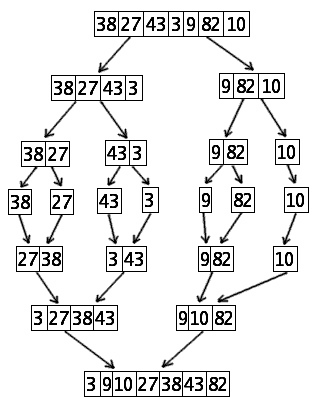
\includegraphics[scale=0.5]{mergesort.png}
      \resizebox{!}{7cm}{
        \begin{tikzpicture}[every node/.style={},>=stealth']
          \node (n1) at (0,0.5) {$\{38,27,43,3,9,82,10\}$}; \node
          (n11) at (-2,-1){$\{38,27,43,3\}$}; \node (n111) at (-3,-2)
          {$\{38,27\}$}; \node (n1111) at (-3.5,-3) {$\{38\}$}; \node
          (n1112) at (-2.5,-3) {$\{27\}$}; \node (n111bis) at (-3,-4)
          {$\{27,38\}$}; \node (n112) at (-1,-2) {$\{43,3\}$}; \node
          (n1121) at (-1.5,-3) {$\{43\}$}; \node (n1122) at (-0.5,-3)
          {$\{3\}$}; \node (n112bis) at (-1,-4) {$\{3,43\}$}; \node
          (n12) at (2,-1) {$\{9,82,10\}$}; \node (n121) at (1,-2)
          {$\{9,82\}$}; \node (n1211) at (0.5,-3) {$\{9\}$}; \node
          (n1212) at (1.5,-3) {$\{82\}$}; \node (n121bis) at (1,-4)
          {$\{9,82\}$}; \node (n122) at (3,-2) {$\{10\}$}; \node
          (n1221) at (3,-3) {$\{10\}$}; \node (n122bis) at (3,-4)
          {$\{10\}$}; \node (n11bis) at (-2,-5) {$\{3,27,38,43\}$};
          \node (n12bis) at (2,-5) {$\{9,10,82\}$}; \node (n1bis) at
          (0,-6.5) {$\{3,9,10,27,38,43,82\}$}; \path (n1.south) edge
          (n11.north); \path (n11.south) edge (n111.north); \path
          (n111.south) edge (n1111.north); \path (n111.south) edge
          (n1112.north); \path (n1111.south) edge (n111bis.north);
          \path (n1112.south) edge (n111bis.north); \path
          (n1121.south) edge (n112bis.north); \path (n1122.south) edge
          (n112bis.north); \path (n111bis.south) edge (n11bis.north);
          \path (n112bis.south) edge (n11bis.north); \path
          (n11bis.south) edge (n1bis.north); \path (n12bis.south) edge
          (n1bis.north); \path (n11.south) edge (n112.north); \path
          (n112.south) edge (n1121.north); \path (n112.south) edge
          (n1122.north); \path (n12.south) edge (n121.north); \path
          (n12.south) edge (n122.north); \path (n121.south) edge
          (n1211.north); \path (n121.south) edge (n1212.north); \path
          (n1211.south) edge (n121bis.north); \path (n1212.south) edge
          (n121bis.north); \path (n122.south) edge (n1221.north);
          \path (n1221.south) edge (n122bis.north); \path
          (n121bis.south) edge (n12bis.north); \path (n122bis.south)
          edge (n12bis.north);
      
          \path (n1.south) edge (n12.north);
        \end{tikzpicture}}%
    \end{center}
  \end{example}
\end{frame}

\begin{frame}[fragile]{Exemple de Divide-and-Conquer}
  \framesubtitle{Tri rapide}

  \begin{algorithm}[H]
    \DontPrintSemicolon \SetKwProg{Fn}{Function}{}{}
    \SetKwFunction{DandC}{quick\_sort} \SetKwFunction{simple}{simple}
    \SetKwFunction{dividef}{partition} \SetKwFunction{merge}{merge}
    \SetKwFunction{pivot}{pivot} \Fn{\DandC{$E$,$g$,$d$}}{
      \If{$d > g$}{ $p \leftarrow$ \pivot{$E$}\;
        \dividef{$E$,$g$,$d$,$p$}\; \DandC{$E$,$g$,$p-1$}\;
        \DandC{$E$,$p+1$,$d$}\; } }
  \end{algorithm}
\end{frame}

\begin{frame}
  \frametitle{Exemple de Divide-and-Conquer}

  \begin{example}[Tri rapide]
    \begin{center}
      % 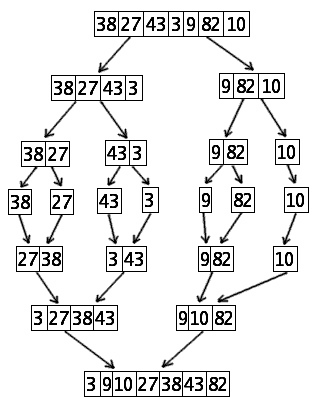
\includegraphics[scale=0.5]{mergesort.png}
      % \resizebox{!}{7cm}{
      % \begin{tikzpicture}[every node/.style={},>=stealth']
      %   \node (n1) at (0,0.5) {$\{38,27,43,3,\mathbf{9},82,10\}$};
      %   \node (n11) at (-3,-1){$\{\mathbf{3},9\}$};
      %   \node (n111) at (-4,-2) {$\{3\}$};
      %   \node (n112) at (-2,-2) {$\{9\}$};
      %   \node (n12) at (3,-1) {$\{\mathbf{38},27,43,82,10\}$};
      %   \node (n121) at (1,-2) {$\{\mathbf{27},10,38\}$};
      %   \node (n1211) at (0,-3) {$\{\mathbf{27},10\}$};
      %   \node (n12111) at (-0.5,-4) {$\{10\}$};
      %   \node (n12112) at (0.5,-4) {$\{27\}$};
      %   \node (n1211bis) at (0,-5) {$\{\mathbf{27},10\}$};
      %   \node (n1212) at (2,-3) {$\{38\}$};
      %   \node (n121bis) at (1,-6) {$\{10,27,38\}$};
      %   \node (n122) at (5,-2) {$\{43,82\}$};
      %   \node (n1221) at (4,-3) {$\{43\}$};
      %   \node (n1222) at (6,-3) {$\{82\}$};
      %   \node (n122bis) at (5,-4) {$\{43,82\}$};
      %   \node (n11bis) at (-3,-3) {$\{3,9\}$};
      %   \node (n12bis) at (3,-7) {$\{10,27,38,43,82\}$};
      %   \node (n1bis) at (0,-8.5) {$\{3,9,10,27,38,43,82\}$};
      %   \path (n1.south) edge (n11.north);
      %   \path (n11.south) edge (n111.north);
      %   \path (n111.south) edge (n11bis.north);
      %   \path (n112.south) edge (n11bis.north);
      %   \path (n11bis.south) edge (n1bis.north);
      %   \path (n12bis.south) edge (n1bis.north);
      %   \path (n11.south) edge (n112.north);
      %   \path (n12.south) edge (n121.north);
      %   \path (n12.south) edge (n122.north);
      %   \path (n121.south) edge (n1211.north);
      %   \path (n121.south) edge (n1212.north);
      %   \path (n1211.south) edge (n12111.north);
      %   \path (n1211.south) edge (n12112.north);
      %   \path (n12111.south) edge (n1211bis.north);
      %   \path (n12112.south) edge (n1211bis.north);
      %   \path (n1211bis.south) edge (n121bis.north);
      %   \path (n1212.south) edge (n121bis.north);
      %   \path (n122.south) edge (n1222.north);
      %   \path (n1222.south) edge (n122bis.north);
      %   %   \path (n1211.south) edge (n121bis.north);
      %   %   \path (n1212.south) edge (n121bis.north);
      %   \path (n122.south) edge (n1221.north);
      %   \path (n1221.south) edge (n122bis.north);
      %   \path (n121bis.south) edge (n12bis.north);
      %   \path (n122bis.south) edge (n12bis.north);
      
      %   \path (n1.south) edge (n12.north);
      % \end{tikzpicture}}%

      \resizebox{!}{7cm}{
        \begin{tikzpicture}[every node/.style={},>=stealth']
          \node (n1) at (0,0.5) {$\{38,27,43,3,\mathbf{9},82,10\}$};
          \node (n11) at (-3,-1){$\{3\}$}; \node (n111) at (-4,-2)
          {$\{3\}$}; \node (n112) at (-2,-2) {$\{9\}$}; \node (n12) at
          (3,-1) {$\{\mathbf{38},27,43,82,10\}$}; \node (n121) at
          (1,-2) {$\{\mathbf{27},10,38\}$}; \node (n1211) at (0,-3)
          {$\{\mathbf{27},10\}$}; \node (n12111) at (-0.5,-4)
          {$\{10\}$}; \node (n12112) at (0.5,-4) {$\{27\}$}; \node
          (n1211bis) at (0,-5) {$\{\mathbf{27},10\}$}; \node (n1212)
          at (2,-3) {$\{38\}$}; \node (n121bis) at (1,-6)
          {$\{10,27,38\}$}; \node (n122) at (5,-2) {$\{43,82\}$};
          \node (n1221) at (4,-3) {$\{43\}$}; \node (n1222) at (6,-3)
          {$\{82\}$}; \node (n122bis) at (5,-4) {$\{43,82\}$}; \node
          (n11bis) at (-3,-3) {$\{3,9\}$}; \node (n12bis) at (3,-7)
          {$\{10,27,38,43,82\}$}; \node (n1bis) at (0,-8.5)
          {$\{3,9,10,27,38,43,82\}$}; \path (n1.south) edge
          (n11.north); \path (n11.south) edge (n111.north); \path
          (n111.south) edge (n11bis.north); \path (n112.south) edge
          (n11bis.north); \path (n11bis.south) edge (n1bis.north);
          \path (n12bis.south) edge (n1bis.north); \path (n11.south)
          edge (n112.north); \path (n12.south) edge (n121.north);
          \path (n12.south) edge (n122.north); \path (n121.south) edge
          (n1211.north); \path (n121.south) edge (n1212.north); \path
          (n1211.south) edge (n12111.north); \path (n1211.south) edge
          (n12112.north); \path (n12111.south) edge (n1211bis.north);
          \path (n12112.south) edge (n1211bis.north); \path
          (n1211bis.south) edge (n121bis.north); \path (n1212.south)
          edge (n121bis.north); \path (n122.south) edge (n1222.north);
          \path (n1222.south) edge (n122bis.north);
          % \path (n1211.south) edge (n121bis.north);
          % \path (n1212.south) edge (n121bis.north);
          \path (n122.south) edge (n1221.north); \path (n1221.south)
          edge (n122bis.north); \path (n121bis.south) edge
          (n12bis.north); \path (n122bis.south) edge (n12bis.north);
      
          \path (n1.south) edge (n12.north);
        \end{tikzpicture}}%
  
    \end{center}
  \end{example}
\end{frame}

\begin{frame}[allowframebreaks]
  \frametitle{Complexité en temps}

  Soit $T(n)$ la complexité en temps pour une donnée de taille $n$,
  alors :

  \begin{equation}
    \label{eq:3}
    T(n) =
    \begin{cases}
      AS(n) & \text{ si } n \leq n_0\\
      \sum_{i=1}^k T(n_i) + D(n) + F(n) & \text{ sinon }
    \end{cases}
  \end{equation}
 
  où

  \begin{itemize}
  \item $AS(n)$ est la complexité en temps de l’algorithme
  \item $D(n)$ est la complexité en temps de la décomposition
  \item $F(n)$ est la complexité en temps de la fusion
  \item $n_i = |E_i|$ est la taille du sous problème $E_i$,
    $i \in\{1, 2, \ldots , k\}$
  \end{itemize}

  Dans le cas général on ne peut rien dire de précis sur $T(n)$ mais
  il existe de nombreux résultats suivant les valeurs de $AS(n)$,
  $D(n)$ et $F(n)$ et la nature de la décomposition \framebreak

  \begin{theorem}
    \label{thm:rec1}
    L’équation de récurrence (où $c$ est une constante positive)
    \begin{equation}
      \label{eq:5}
      T(n) = 
      \begin{cases}
        c & \text{ si } n = 1\\
        T(n/2) + c & \text { si } n \geq 2
      \end{cases}
    \end{equation}
    admet comme solution $T(n) \in \Theta(\log_2n)$
  \end{theorem}

  \framebreak

  \begin{exampleblock}{Remarques}
    \begin{itemize}
    \item Valide si $T(n) \leq \ldots$ (resp. $\geq$) avec
      $\mathcal{O}$ (resp. $\Omega$) à la place de $\Theta$
    \item Valide pour $n \leq n_0$ au lieu de $n = 1$ et $n > n_0$ à
      la place de $n \geq 2$
    \item Correspond à une stratégie récursive
      \begin{itemize}
      \item résoudre un problème de taille $n$ en ré-appliquant la
        même méthode sur le même problème de taille $n/2$ via un
        travail en $\mathcal{O}(1)$
      \end{itemize}
    \item Si, dans un algo, on fait apparaître un paramètre dont
      dépend le nombre d’appels récursifs ou le nombre de boucles et
      dont la taille est divisée par $2$ à chaque étape, il y aura
      $\Theta(\log_2n)$
    \end{itemize}
  \end{exampleblock}

  \framebreak

  \begin{theorem}
    \label{thm:rec2}
    L’équation de récurrence (où $a$, $b$ et $c$ sont des constantes
    positives)
    \begin{equation}
      \label{eq:6}
      T(n) = 
      \begin{cases}
        a & \text{ si } n = 1\\
        c\cdot T(n/b) + a\cdot n & \text { si } n \geq 2
      \end{cases}
    \end{equation}
    admet comme solutions
    \begin{equation}
      T(n) \in
      \begin{cases}
        \Theta(n) & \text{ si } b > c\\
        \Theta(n\cdot\log n) & \text{ si } b=c\\
        \Theta(n^{\log_bc}) & \text{ si } b < c
      \end{cases}
      \label{eq:7}
    \end{equation}

  \end{theorem}

  \framebreak
  \begin{exampleblock}{Remarques}
    \begin{itemize}
    \item Valide si $T(n) \leq \ldots$ (resp. $\geq$) avec
      $\mathcal{O}$ (resp. $\Omega$) à la place de $\Theta$
    \item Valide pour $n \leq n_0$ au lieu de $n = 1$ et $n > n_0$ à
      la place de $n \geq 2$
    \item Correspond à une stratégie récursive
      \begin{itemize}
      \item résoudre un problème de taille $n$ en le décomposant en
        $c$ sous-problèmes de taille $n/b$ puis résoudre ces $c$
        sous-problèmes de telle sorte que la décomposition ainsi que
        la construction de la solution globale se fasse en $\Theta(n)$
      \end{itemize}
      \alert{\item À retenir absolument : le cas
        $T(n) = 2\cdot T(n/2) + a\cdot n$ qui donne
        $T(n) \in \Theta(n\cdot \log n)$}
    \end{itemize}
  \end{exampleblock}

  \framebreak

  On peut généraliser le Théorème~\ref{thm:rec2} :
  
  \begin{theorem}
    \label{thm:rec3}
    L’équation de récurrence (où $a$, $b$ et $c$ sont des constantes
    positives)
    \begin{equation}
      \label{eq:8}
      T(n) = 
      \begin{cases}
        a & \text{ si } n = 1\\
        c\cdot T(n/b) + a\cdot n^k & \text { si } n \geq 2
      \end{cases}
    \end{equation}
    admet comme solutions
    \begin{equation}
      T(n) \in
      \begin{cases}
        \Theta(n^k) & \text{ si } b^k > c\\
        \Theta(n^k\cdot\log n) & \text{ si } b^k = c\\
        \Theta(n^{\log_bc}) & \text{ si } b^k < c
      \end{cases}
      \label{eq:9}
    \end{equation}

  \end{theorem}

  \framebreak
  \begin{exampleblock}{Remarques}
    \begin{itemize}
    \item Valide si $T(n) \leq \ldots$ (resp. $\geq$) avec
      $\mathcal{O}$ (resp. $\Omega$) à la place de $\Theta$
    \item Valide pour $n \leq n_0$ au lieu de $n = 1$ et $n > n_0$ à
      la place de $n \geq 2$
    \item Correspond à une stratégie récursive
      \begin{itemize}
      \item résoudre un problème de taille $n$ en le décomposant en
        $c$ sous-problèmes de taille $n/b$ puis résoudre ces $c$
        sous-problèmes de telle sorte que la décomposition ainsi que
        la construction de la solution globale se fasse en
        $\Theta(n^k)$
      \end{itemize}
    \end{itemize}
  \end{exampleblock}
  \framebreak
  
  \begin{theorem}
    \label{thm:rec4}
    L’équation de récurrence (où $a$, $\alpha$ et $\beta$ sont des
    constantes positives, et $\alpha + \beta \leq 1$)
    \begin{equation}
      \label{eq:10}
      T(n) = 
      \begin{cases}
        a & \text{ si } n = 1\\
        T(\alpha\cdot n) + T(\beta\cdot n) + a\cdot n & \text { si } n
        \geq 2
      \end{cases}
    \end{equation}
    admet comme solutions
    \begin{equation}
      T(n) \in
      \begin{cases}
        \Theta(n) & \text{ si } \alpha + \beta < 1\\
        \Theta(n\cdot\log n) & \text{ si } \alpha + \beta = 1
      \end{cases}
      \label{eq:11}
    \end{equation}

  \end{theorem}

  \framebreak
  \begin{exampleblock}{Remarques}
    \begin{itemize}
    \item Valide si $T(n) \leq \ldots$ (resp. $\geq$) avec
      $\mathcal{O}$ (resp. $\Omega$) à la place de $\Theta$
    \item Valide pour $n \leq n_0$ au lieu de $n = 1$ et $n > n_0$ à
      la place de $n \geq 2$
    \item Correspond à une stratégie récursive
      \begin{itemize}
      \item résoudre un problème de taille $n$ en le décomposant en
        $2$ sous-problèmes de taille $\alpha\cdot n$ et $\beta\cdot n$
        puis résoudre ces $2$ sous-problèmes de telle sorte que la
        décomposition ainsi que la construction de la solution globale
        se fasse en $\Theta(n)$
      \end{itemize}
    \end{itemize}
  \end{exampleblock}

  \framebreak

  \begin{itemize}
  \item On peut considérer ces résultats comme des pistes de recherche
    de stratégies de résolution de problèmes
    \begin{itemize}
    \item e.g., si on cherche à résoudre un problème de taille $n$ en
      $\mathcal{O}(n\cdot\log n)$ en temps, on peut essayer de le
      décomposer récursivement en $2$ sous problèmes de taille $n/2$
      de telle sorte que la décomposition et la construction de la
      solution globale se fasse en $\mathcal{O}(n)$ (cf. tri fusion)
    \end{itemize}
  \item Pour l’implémentation il faudra déterminer expérimentalement
    un seuil $n_0$ en dessous duquel un algorithme plus simple est
    globalement plus efficace
  \item La complexité asymptotique dépend essentiellement des
    complexités de la décomposition et de la fusion
  \item Un bon équilibrage entre les sous-problèmes est souvent gage
    d’une bonne complexité (cf. tri fusion)
  \item Mais la meilleure complexité n’est pas forcément obtenue avec
    un parfait équilibrage, elle l’est quand la décomposition permet
    de réduire substantiellement la taille du problème (soit
    directement, soit par sous-problèmes) de $n$ à $\alpha\cdot n$
    (cf. Théorème~\ref{thm:rec2} et Théorème~\ref{thm:rec4}),
    \alert{mais c'est difficile à obtenir !}

  \end{itemize}
  
\end{frame}

\newcommand{\drawEC}{%
  \node[point] (n1) at (0,0) {}; \node[point] (n2) at (2,-2) {};
  \node[point] (n3) at (5,-3) {}; \node[point] (n4) at (6,-0.5) {};
  \node[point] (n5) at (6,0.75) {}; \node[point] (n6) at (3.5,1.75)
  {}; \node[point] (n7) at (1,1.5) {}; \draw[thick] (n1) -- (n2) --
  (n3) -- (n4) -- (n5) -- (n6) -- (n7) -- (n1);
    
  \node[point] (n8) at (4.25,0.5) {}; \node[point] (n9) at (4.5,-0.75)
  {}; \node[point] (n10) at (6.5,-1.75) {}; \node[point] (n11) at
  (10,-1.25) {}; \node[point] (n12) at (11,0.5) {}; \node[point] (n13)
  at (10,2.5) {}; \node[point] (n14) at (6.5,3) {}; \node[point] (n15)
  at (5,2) {}; \draw[thick] (n8) -- (n9) -- (n10) -- (n11) -- (n12) --
  (n13) -- (n14) -- (n15) -- (n8); }

  \begin{frame}[b]{Divide-and-Conquer pour EC}
    \framesubtitle{Algorithme de Shamos (1977)}
  
    \only<1>{
      \begin{itemize}
      \item Décomposer $E = \{p_1, \ldots , p_n\}$ en
        $E_1 = \{p_1, \ldots , p_{n/2}\}$ et
        $E_2 = \{p_{n/2+1}, \ldots, p_n\}$
      \item Calculer récursivement $EC(E_1)$ et $EC(E_2)$
      \item Construire l’enveloppe convexe de $E$ à partir de celles
        de $E_1$ et $E_2$ :
        \begin{equation}
          EC(E) = EC( EC(E_1) \cup EC(E_2) )\label{eq:shamos1}
        \end{equation}
      \end{itemize}
    }

    \only<2>{ Résoudre l'équation (\ref{eq:shamos1}) nécessite de
      \begin{itemize}
      \item Déterminer les deux segments $T_b$ et $T_h$
      \item Supprimer des sommets « intérieurs »
      \item Raccorder aux extrémités de $T_b$ et $T_h$
      \end{itemize}
    }

    \only<3>{
      \begin{itemize}
      \item Choix d’un point $p \in EC(E_1)$ (donc $p \in EC(E)$) en
        $\mathcal{O}(1)$
      \item Si $p \in EC(E_2)$ -- vérifiable en $\mathcal{O}(|E_2|)$--
        alors, comme les sommets de $E_1$ et ceux de $E_2$ sont
        polairement ordonnés autour de $p$, il suffit de « fusionner »
        les deux listes
      \item Appliquer le balayage de Graham (cf. TD) sur la liste
        obtenue -- $\mathcal{O}(|E_1| + |E_2|)$
      \end{itemize}
    }

    \only<4>{
      \begin{itemize}
      \item Si $p \notin EC(E_2)$ alors $EC(E_2)$ est contenue dans un
        secteur angulaire $\alpha < \pi$ d’origine $p$, s'appuyant sur
        les points $b$ et $h$ de $EC(E_2)$, en $\mathcal{O}(|E_2|)$
      \item Eliminer les points intérieurs à $\alpha$ sur $EC(E_1)$ et
        ceux situés entre $h$ et $b$ sur $EC(E_2)$
      \item Les points restants sont polairement ordonnés par rapport
        à $p$
      \item Fusionner ces points puis d’appliquer un balayage de
        Graham -- en $\mathcal{O}(n)$
      \end{itemize}
    }
  

    \vfill
  
  \begin{center}
    \resizebox{!}{4cm}{%
      \begin{tikzpicture}[point/.style={fill=black,draw,circle},extended
        line/.style={shorten >=-####1}, extended line/.default=1cm]
        \drawEC{} \only<2->{ \draw[dashed] (n7) edge node[above]
          {$T_h$} (n14); \draw[dashed] (n3) edge node[below] {$T_b$}
          (n11); }

        \node[left = 0.5 of n1] {$EC(E_1)$}; \node[right = 0.5 of n12]
        {$EC(E_2)$};

        \only<3>{ \node[point,fill=blue] (p) at (5.25,0.5) {};
          \node[below = 0.1 of p] {$p$}; }
      
        \only<4>{ \node[point,fill=blue] (p) at (2.75,0.75) {};
          \node[below = 0.1 of p] {$p$}; \draw [extended
          line=1cm,dotted,draw=blue,very thick] (p) -- (n14); \draw
          [extended line=3.5cm,dotted,draw=blue,very thick] (p) --
          (n9);
          \node[below = 0.1 of n14] (h){$h$};
          \node[above right= 0.1 of n9] (b){$b$};
        }
      \end{tikzpicture}
    }
    % \includegraphics[height=3cm]{shamos1.pdf}
  \end{center}
  
\end{frame}

\begin{frame}[allowframebreaks]{Divide-and-Conquer pour EC}
  \framesubtitle{Algorithme d'Eddy-Floyd}

  \begin{itemize}
  \item Calcul des points extrémaux, $p_m$ et $p_M$ (d’abscisse
    minimale et maximale) de $E = \{p_1, \ldots , p_n\}$
  \item Détermination de $E_1$ et $E_2$, ensembles de points situés
    respectivement à droite et à gauche du segment $[p_mp_M]$
  \item Calcul de l’enveloppe inférieure (droite) sur $E_1$ de $p_m$ à
    $p_M$ (dans le sens direct) puis, par la même méthode, calcul de
    l’enveloppe supérieure (gauche) sur $E_2$ de $p_M$ à $p_m$ (dans
    le sens direct)
  \item L’enveloppe finale est obtenue par raccordement de ces deux
    sous-enveloppes
  \end{itemize}

  \framebreak

  Le calcul de l’enveloppe inférieure se fait en considérant $E_1$ :
  \begin{itemize}
  \item détermination d’un point $p$ de $E_1$ tel que $p \in EC(E)$,
    par exemple le point situé à plus grande distance du segment
    $[p_mp_M]$ (ou le point $p$ tel que l’aire du triangle
    $[p_m,p,p_M]$ soit maximale)
  \item Application récursive sur les sous-ensembles de points
    $E_{11}$ et $E_{12}$ de $E_1$ situés respectivement à droite des
    segments $[p_mp]$ et $[pp_M]$ (idem pour $E_2$)
  \end{itemize}
  
  \begin{center}
    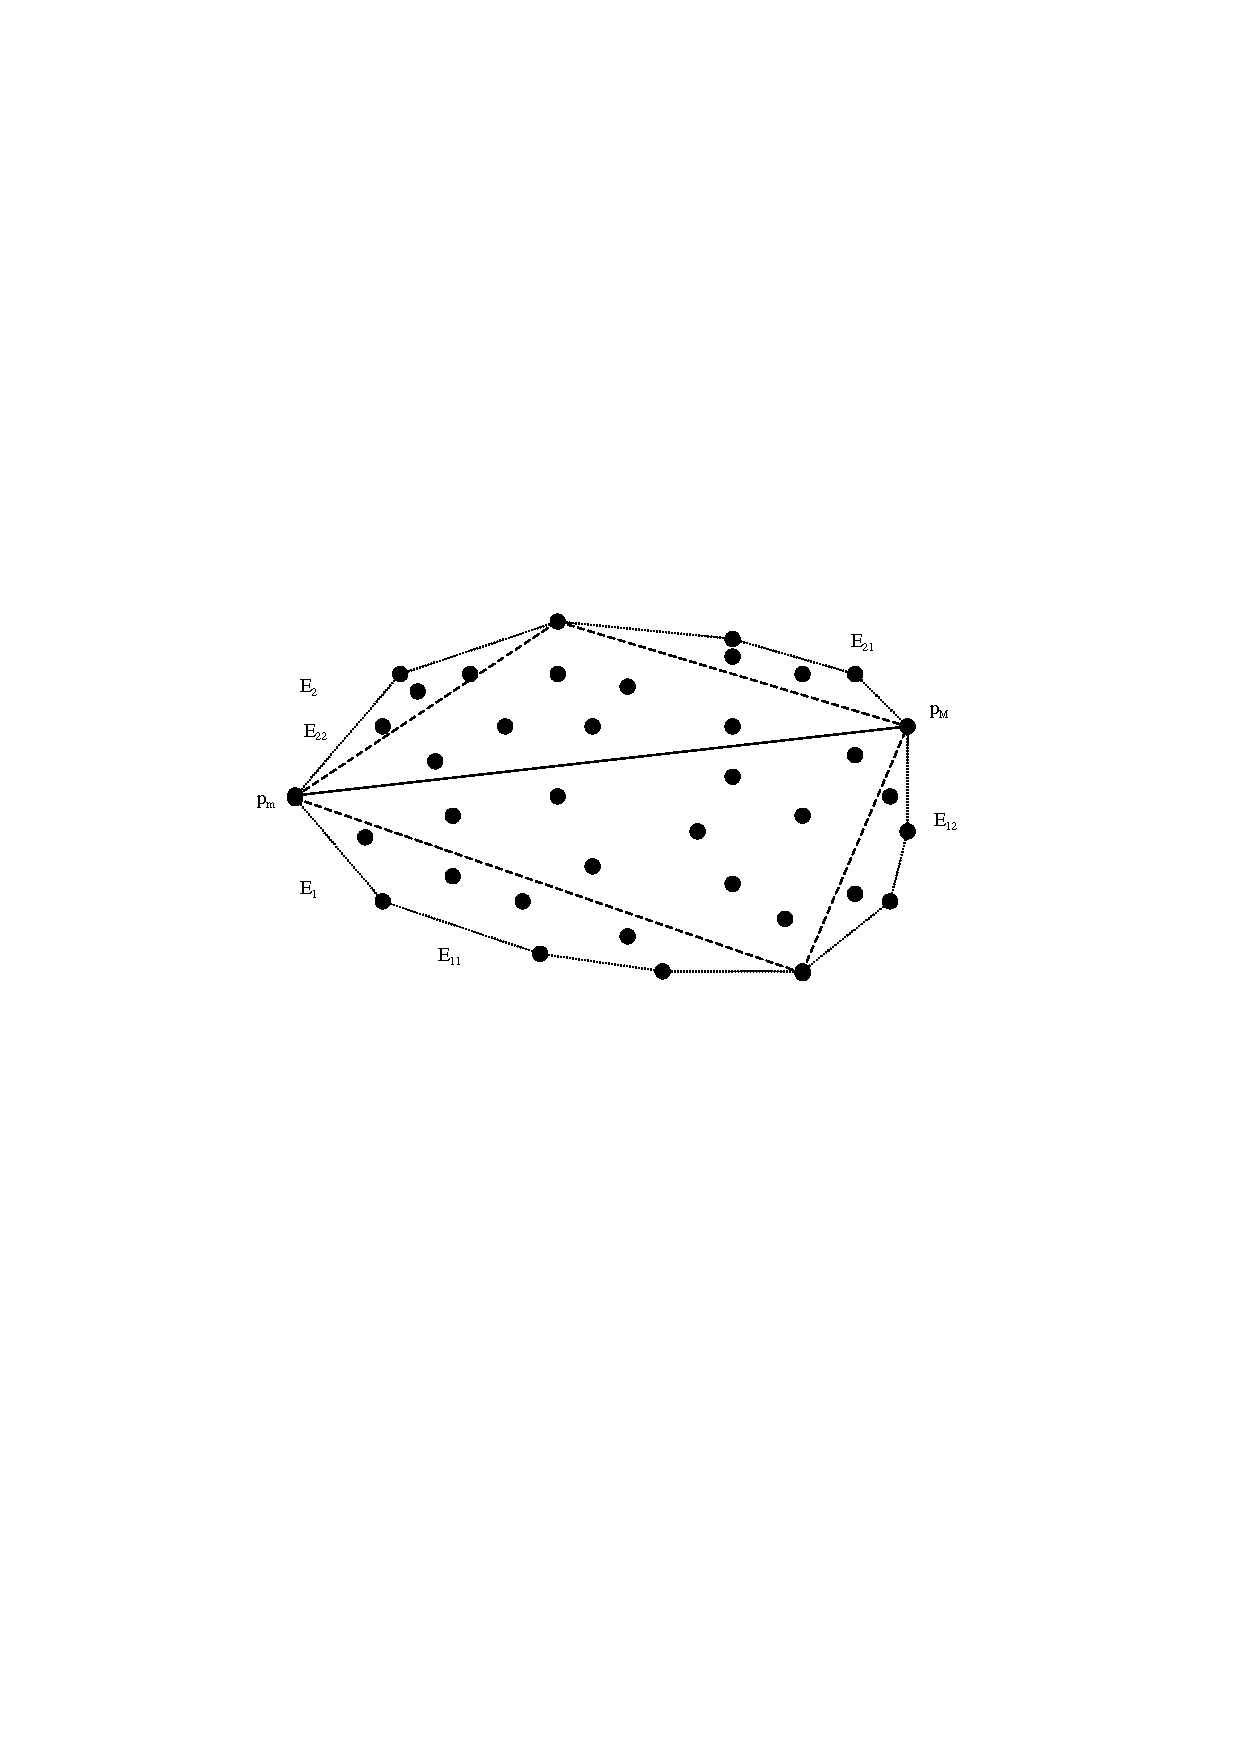
\includegraphics[height=3.5cm]{eddyfloyd.pdf}
  \end{center}

  \framebreak

  \begin{itemize}
  \item L’étape préliminaire se fait en $\Theta(n)$ (calcul d’un
    minimum et d’un maximum)
  \item L’étape courante qui consiste à trouver $p$ et à déterminer
    les deux sous-ensembles extérieurs au triangle se fait en
    $\mathcal{O}(n)$
  \item Chaque étape, sauf la première, trouve exactement un point de
    l’enveloppe convexe donc globalement l’algorithme est en
    $\mathcal{O}(n \cdot e)$ où $e = |EC(E)|$
  \end{itemize}
\end{frame}

\begin{frame}{Divide-and-Conquer pour EC}
  \framesubtitle{Remarques}

  \begin{itemize}
  \item L’algorithme de Shamos s’apparente au \structure{Tri par
      Fusions} alors que l’algorithme d’Eddy-Floyd est très proche du
    \structure{Tri Rapide}
  \item Peut-on s’inspirer d’autres algorithmes de Tri pour trouver
    d’autres algorithmes de construction de l’EC dans le plan ? Et
    dans l’espace ?
  \item L’algorithme d’Eddy-Floyd est plus intéressant que celui de
    Shamos si l’on sait qu’il y aura peu de points sur $EC(E)$

  \end{itemize}
\end{frame}


\begin{frame}{Avantages et Inconvénients du Divide-and-Conquer}

  \begin{itemize}
  \item \structure{Simplicité} de l’approche et de nombreux problèmes
    se décomposent naturellement
  \item Preuve immédiate : \structure{finitude} (car appels récursifs
    sur des problèmes de tailles inférieures) et \structure{validité}
    (preuve par récurrence sur la taille) à condition que la
    décomposition et la fusion soient irréprochables
  \item\structure{ Facilité de programmation} dans un langage
    disposant de la récursivité
  \item \structure{Parallélisme} possible quand les sous problèmes
    peuvent être résolus de façons indépendantes
  \item Un parfait équilibrage n’est pas toujours facile à obtenir, il
    peut être facilité par un \structure{prétraitement}, un tri
    préalable des données, par exemple
  \item La récursivité peut amener des redondances dans le sens où les
    mêmes calculs peuvent être effectués plusieurs fois comme dans
    l’algorithme récursif résultant directement de l’équation de
    récurrence définissant la suite de FIBONACCI
  \item La\structure{ détermination du seuil idéal $n_0$} dépend bien
    sûr du problème, de l’algorithme, de l’implémentation
  \end{itemize}
\end{frame}

\section{Pré-traitement}

\begin{frame}[allowframebreaks]{Pré-traitement}

  On trouve aussi les appellations \structure{Pré-Conditionnement} ou
  \structure{\emph{Preprocessing}}

  \begin{alertblock}{Principe}
    \it Il s’agit d’organiser, d’ordonner, de structurer, \ldots les
    données pour accélérer les traitements ultérieurs
  \end{alertblock}
  
  \begin{example}
    Imaginez un dictionnaire dont les mots sont listés dans un ordre
    quelconque\ldots
    
    La recherche d’un mot dans un dictionnaire est bien sûr efficace
    grâce au classement alphabétique, en gros en
    $\mathcal{O}(\log\log n)$ en moyenne, c’est en gros une
    \structure{Recherche par Interpolation}.
    
    Et le mot «~\emph{ordinateur}~» ne signifie t’il pas aussi «~qui
    ordonne~», «~qui met en ordre~» ?
  \end{example}

  \framebreak

  Cette approche est capitale en informatique si l’on doit résoudre le
  même type de problèmes ou répondre à des questions identiques sur
  les mêmes données ou des données évoluant dans le temps.

  On peut analyser algorithmiquement les stratégies de résolution de
  ce type de problèmes sous trois aspects :
  \begin{itemize}
  \item \structure{Temps de Prétraitement} (Preprocessing Time),
    c’est-à-dire la complexité en temps de l’algorithme structurant
    les données
  \item \structure{Taille de la Structure de Données} utilisée pour
    stocker les données
  \item \structure{Temps de Résolution} (Query Time), c'est-à-dire
    temps de calcul nécessaire à la résolution du problème ou pour
    obtenir la réponse à une question
  \end{itemize}

  Examinons cette stratégie sur quelques problèmes
  
\end{frame}

\begin{frame}[allowframebreaks]{Pré-traitement sur un problème de
    recherche}

  \begin{definition}[Recherche]
    \begin{description}
    \item [Données] $E = \{e(1), e(2), \ldots , e(n)\}$, un ensemble
      de $n$ éléments
    \item [Question] Tester si un élément, $x$, de même nature que
      ceux de $E$, est dans $E$ et, éventuellement, si oui, le
      supprimer $x$ de $E$, et sinon le rajouter à $E$
    \end{description}
  \end{definition}

  Toute structure de données permettant de réaliser ces opérations
  s’appelle un \structure{Dictionnaire}

  \begin{itemize}
  \item Un tri préalable, temps de prétraitement en $\Theta(n\log n)$
    et structure de taille $\Theta(n)$, permet la \structure{Recherche
      Dichotomique} (ou Binaire ou Logarithmique) en $\Theta(\log_2n)$
  \item $E$ est alors représenté par un \structure{tableau trié}, ce
    qui pose des problèmes pour la suppression et l’insertion car ces
    opérations ne sont faisables qu’en $\mathcal{O}(n)$ dans le pire
    cas
  \end{itemize}

  \framebreak

  \begin{center}
    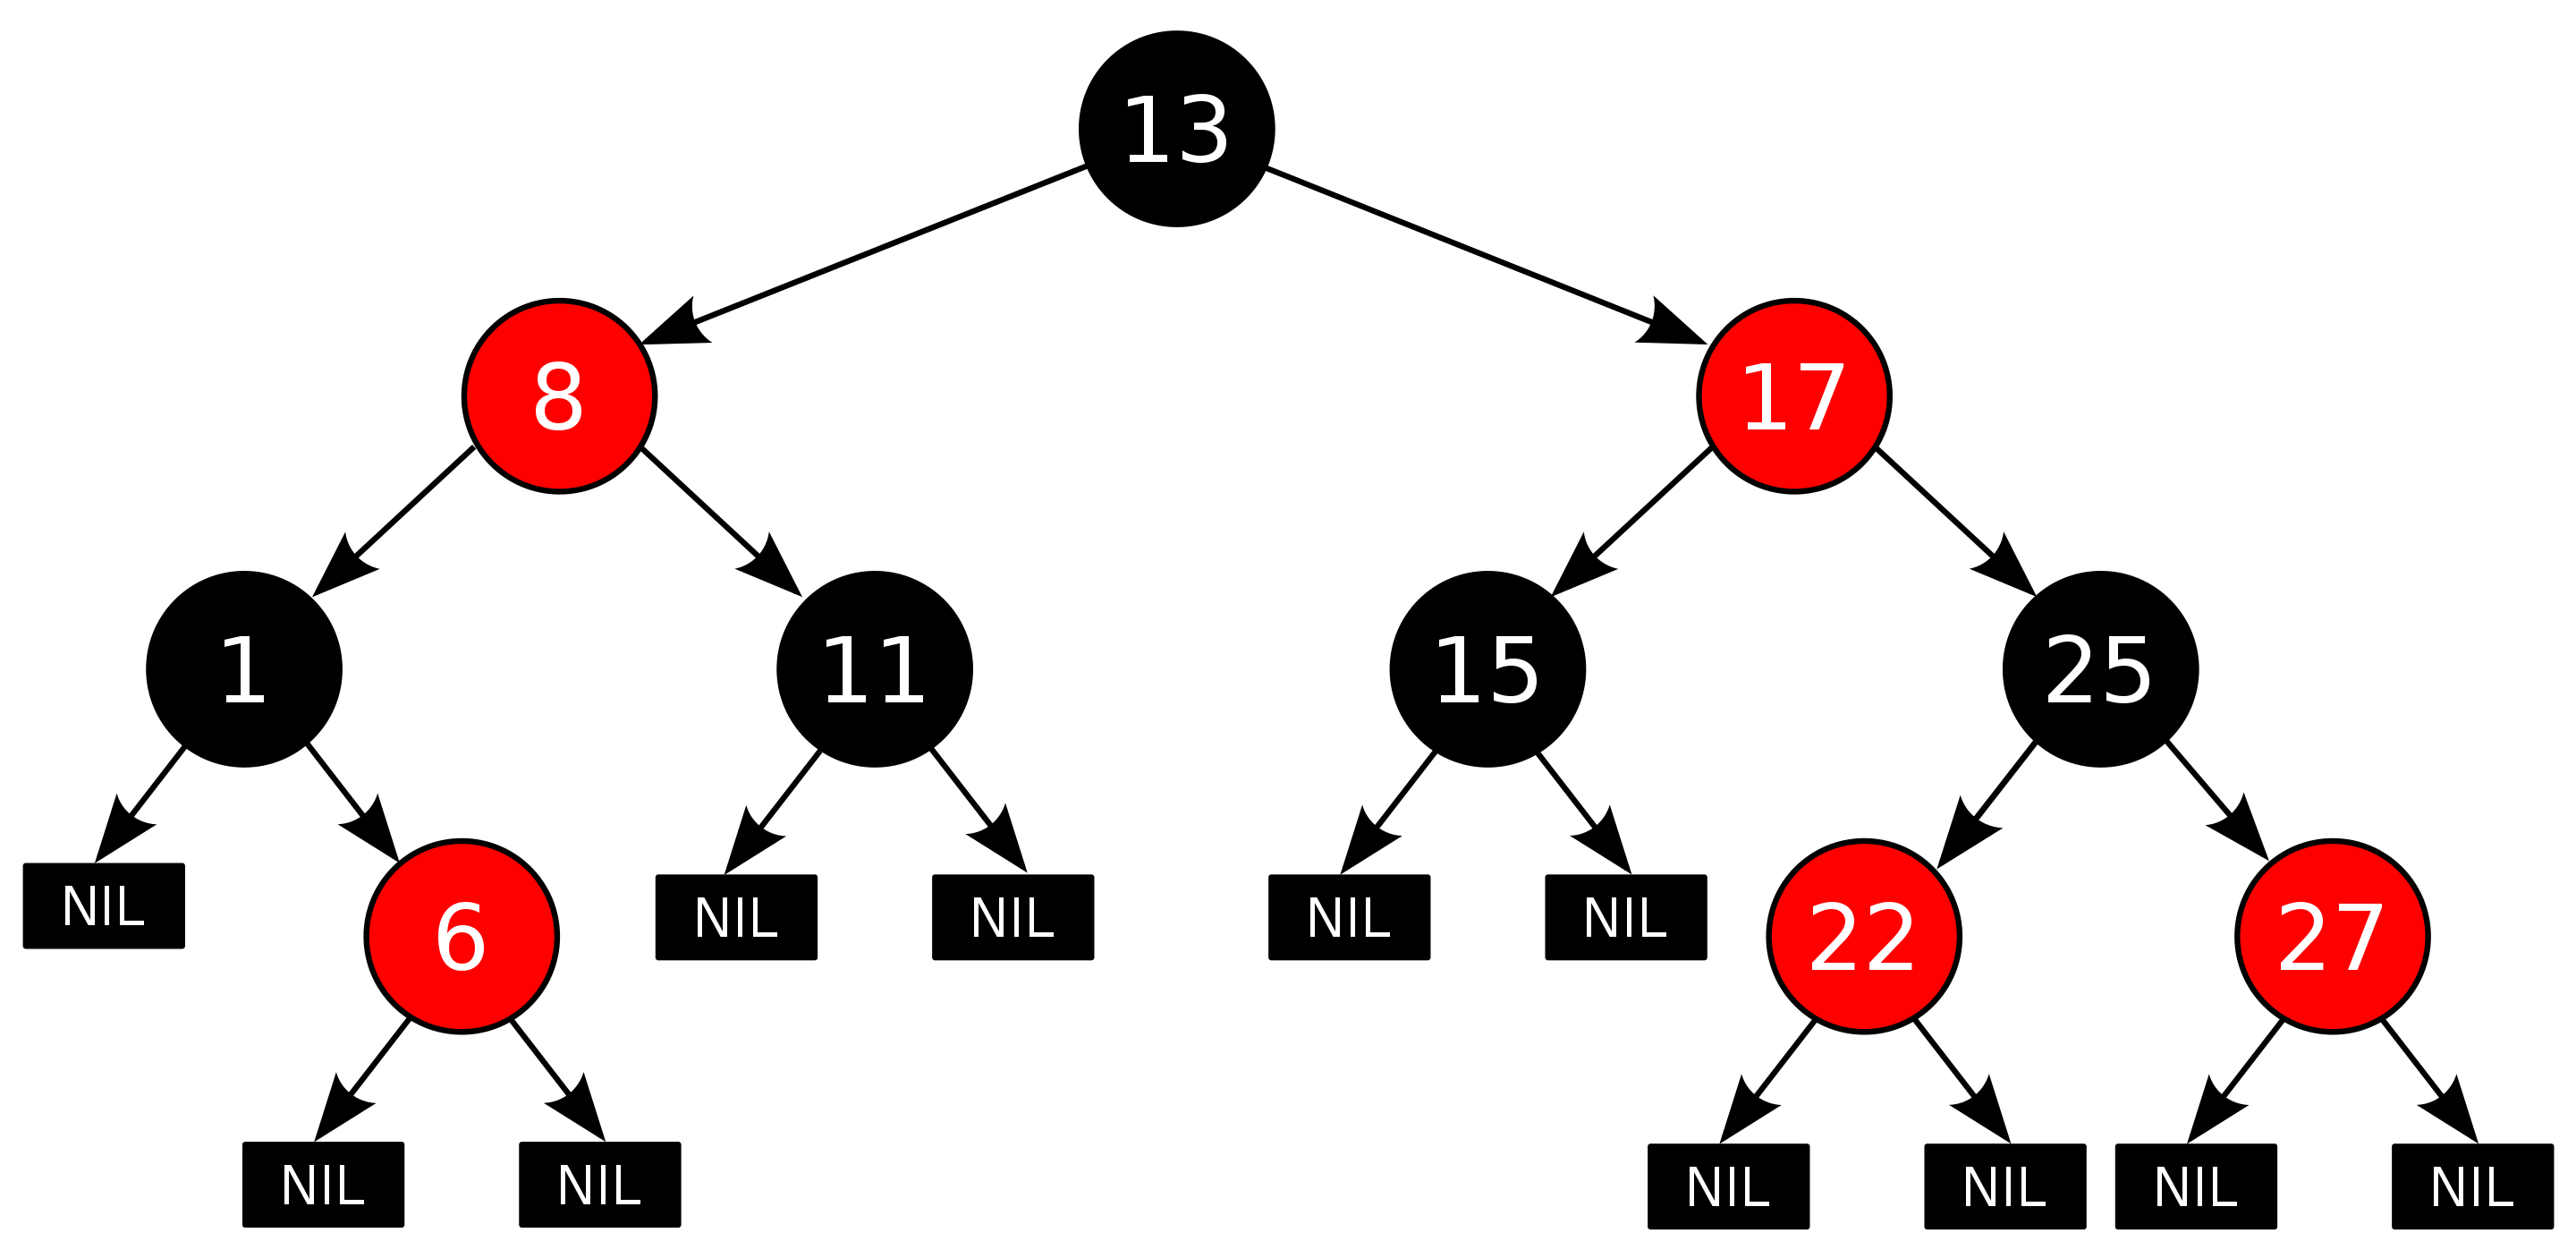
\includegraphics[height=3cm]{redblacktree}
  \end{center}

  Les meilleures structures pour ce problème sont les
  \structure{Arborescences} (ou \structure{Arbres}, en Informatique)
  \structure{de Recherche Equilibrées} (AVL, Arbres 2-3, B-Arbres,
  Arbres Rouges-Noirs, \ldots) pour lesquelles on a (à une constante
  près) :

  \begin{itemize}
  \item un prétraitement en $n\cdot\log n$
  \item une structure de taille $n$
  \item la recherche (et la suppression, et l’insertion) en au plus
    $\log n$
  \end{itemize}

  On peut montrer que ces performances sont optimales, à une constante
  près
\end{frame}

\begin{frame}[allowframebreaks]{Pré-traitement pour P$^\mathsf{4}$}

  \structure{Rappel} : Soit $E = \{p_1, p_2, \ldots , p_n\}$, un
  ensemble de $n$ points du plan, chacun étant donné par ses
  coordonnées $p_i = (x_i, y_i)$, il s’agit de trouver dans $E$ deux
  points dont la distance est minimale

  \begin{itemize}
  \item La recherche exhaustive, qui teste toutes les paires de
    points, donne une solution en $\Theta(n^2)$ en temps et en
    $\Theta(n)$ en espace
  \item Sur des nombres, en dimension $1$, on cherche deux nombres les
    plus proches : se résoud en $\mathcal{O}(n\log n)$
  \item On peut aussi résoudre P$^\mathsf{4}$ dans le plan de façon
    optimale en $\mathcal{O}(n\log n)$
    \begin{itemize}
    \item \structure{Pré-traitement} : tri des points par rapport à
      $x$, puis par rapport à $y$
    \item \structure{Divide-and-Conquer} sur les points triés
    \end{itemize}
  \end{itemize}

\end{frame}

\begin{frame}[allowframebreaks]{Pré-traitement pour P$^\mathsf{4}$
    \insertcontinuationtext}

  \framesubtitle{Principe du Divide-and-Conquer}

  \begin{itemize}
  \item Division de $E$ en deux sous ensembles $E_1$ et $E_2$ de même
    taille, $n/2$, par rapport à $x$
  \item Application récursive de l’algorithme sur $E_1$ et $E_2$
  \item Obtention de deux paires de points les plus proches,
    $\{A_1, B_1\}$ pour $E_1$ et $\{A_2, B_2\}$ pour $E_2$ et donc des
    deux distances correspondantes, $d_1 = d(A_1, B_1)$ et
    $d_2 = d(A_2, B_2)$
  \end{itemize}

  Comment alors déterminer une paire de points les plus proche,
  $\{A, B\}$ et leur distance, $\delta$, dans $E$ ?

  \begin{itemize}
  \item Remarque :
    \begin{itemize}
    \item soit $\{A, B\} = \{A_1, B_1\}$
    \item soit $\{A, B\} = \{A_2, B_2\}$
    \item soit $A$ est dans $E_1$ et $B$ est dans $E_2$
    \end{itemize}
  \end{itemize}
  
  \framebreak
  
  \begin{itemize}
  \item Notons $d = \min (d_1, d_2)$
  \item Où peuvent être $A$ et $B$ dans le dernier cas ?
  \item Soient $p_i$ un point d’abscisse maximale de $E_1$ et $p_j$ un
    point d’abscisse minimale de $E_2$
  \item Notons $D_c$ la droite verticale d’équation
    $x = 1/2\cdot (x_i + x_j)$ et $D_g$ et $D_d$, les deux droites
    verticales d’équations respectives :
    \begin{itemize}
    \item $x = 1/2\cdot (x_i + x_j) - d$, à gauche
    \item $x = 1/2 \cdot (x_i + x_j) + d$, à droite
    \end{itemize}
  \item Il faut alors chercher $A$ et $B$ dans la bande verticale
    centrale de largeur $2d$ située à « cheval » sur $E_1$ et $E_2$
    définie par $D_g$ et $D_d$
  \end{itemize}
\end{frame}

\begin{frame}[allowframebreaks]{Pré-traitement pour P$^\mathsf{4}$ \insertcontinuationtext}
  \framesubtitle{Géométriquement}

  \begin{center}
    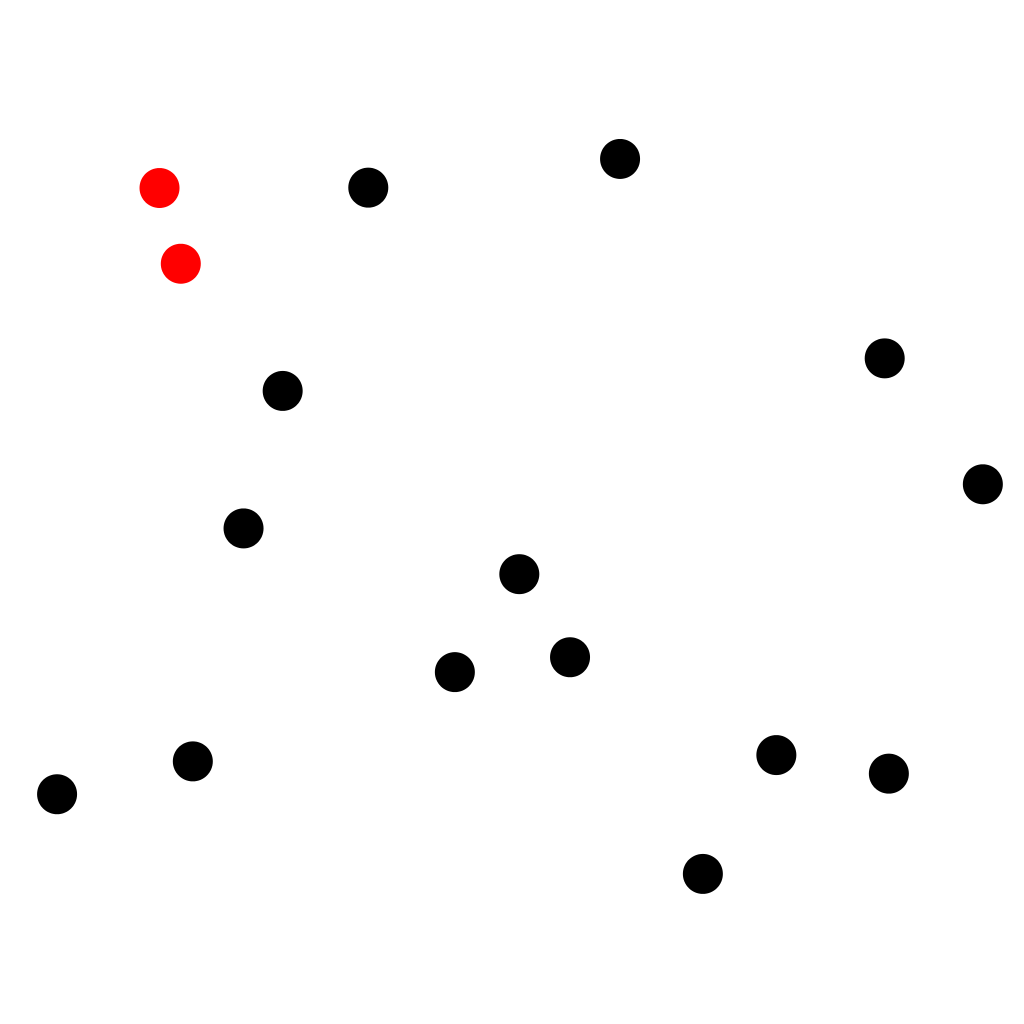
\includegraphics[width=0.8\textwidth]{p4}
  \end{center}
\end{frame}
\begin{frame}[allowframebreaks]{Pré-traitement pour P$^\mathsf{4}$
    \insertcontinuationtext}

  \framesubtitle{Problème : rechercher efficacement, en temps
    linéaire, le points $A$ et $B$ dans la bande verticale centrale}

  \begin{itemize}
  \item Trier par rapport à l’ordonnée ne suffit pas car a priori
    chaque point doit être comparé au pire à $n - 1$ autres points
  \end{itemize}

  
  \begin{theorem}
    S’il y a $n\geq 5$ points dans un carré de coté égal à $d$ alors
    au moins deux d’entre eux sont à une distance $< d$
  \end{theorem}
  \begin{proof}
    Découpons ce carré en quatre carrés, chacun ayant un coté égal à
    $d/2$, alors au moins $2$ points parmi eux, $p$ et $q$, se
    trouvent dans l’un d’entre eux, on a alors :
    
    \begin{equation}
      \label{eq:p4}
      d(p,q) \leq \sqrt{\frac{d^2}{4} + \frac{d^2}{4}} = \sqrt\frac{d^2}{2} = \frac{d}{\sqrt{2}} < d
    \end{equation}

    Ceci montre que pour tout point $p$ de $E_1$ situé entre $D_g$ et
    $D_c$ il n’y aura qu’au plus quatre points de $E_2$ (situés entre
    $D_c$ et $D_d$) à tester
  \end{proof}
\end{frame}
\begin{frame}[allowframebreaks]{Pré-traitement pour P$^\mathsf{4}$
    \insertcontinuationtext}
  \framesubtitle{Algorithme récursif}

  \begin{alertblock}{Principe}
    \begin{itemize}
    \item Tri de E par $x$ croissants puis par $y$ croissants
    \item Construction de la liste $E$
    \item Parcours simultané des listes $E_1$ et $E_2$ et pour chaque
      point $p (x, y)$, vérifiant $x \geq x_g$ si $p \in E_1$ ou
      $x \leq x_d$ si $p \in E_2$, on calcule sa distance aux points
      de l’autre liste ayant une ordonnée plus grande et situés à une
      distance au plus $\delta$, dès qu’une distance plus petite est
      trouvée on la stocke ainsi que les points correspondants
    \item On compare la distance ainsi trouvée à $d_1$ et $d_2$ et la
      réponse est la paire de points correspondant à la distance
      minimale, $\delta$
    \end{itemize}
  \end{alertblock}
  
  \vfill
 
  \bigskip
  
  \begin{algorithm}[H]
    \scriptsize \DontPrintSemicolon \SetKwProg{Fn}{Function}{}{}
    \SetKwFunction{pppp}{$P^4$} \SetKwFunction{simple}{simple}
    \Fn{\pppp{$E$,$1$,$n$;$A$,$B$,$\delta$}}{ \eIf{$n \leq n_0$}{
        \simple{E,1,n;A,B,$\delta$} }{ $m \leftarrow (1 + n)/2$\;
        $E_1 \leftarrow \emptyset$\; $E_2 \leftarrow \emptyset$\;
        \For{$p_i\in E$}{ \leIf{$k_i \leq
            m$}{$E_1 \leftarrow E_1 +
            \{p_i\}$}{$E_2 \leftarrow E_2 + \{p_i\}$}
          \lIf{$k_i = m$}{$i(g) \leftarrow k_i$}
          \lIf{$k_i = m + 1$}{$i(d) \leftarrow k_i$} } \pppp{$E_1$,
          $1$, $m$ ; $A_1$, $B_1$, $d_1$}\; \pppp{$E_2$, $m +1$, $n$ ;
          $A_2$, $B_2$, $d_2$}\; $d \leftarrow \min (d_1, d_2)$\;
        $\delta\leftarrow d$\;
        $x_c \leftarrow 1/2\cdot (x_{i(g)} + x_{i(d)})$\;
        $x_g \leftarrow x_c - d$\; $x_d \leftarrow x_c + d$ } }
  \end{algorithm}
\end{frame}
\begin{frame}[allowframebreaks]{Pré-traitement pour P$^\mathsf{4}$
    \insertcontinuationtext}

  \framesubtitle{Complexité}

  \begin{itemize}
  \item La complexité en espace est en $\Theta(n)$ car l’algorithme ne
    manipule que des structures de tailles $n$
  \item Si l’on veut être rigoureux, il faut y rajouter la taille
    $\Theta(\log n)$, de la pile, invisible à nos yeux, gérant les
    appels récursifs
  \item La complexité en temps, $T(n)$, est en $\Theta(n\log n)$ car,
    en dehors du prétraitement qui est aussi en $\Theta(n\log n)$,
    $T(n)$ vérifie l’équation de récurrence :
    \begin{equation}
      \label{eq:p4cplx}
      T(n) =
      \begin{cases}
        c & \text{ si } n \leq n_0\\
        2\cdot T(n/2) + c\cdot n & \text{ si } n > n_0
      \end{cases}
    \end{equation}
 
  \item La construction des listes $E_1$ et $E_2$ à partir de $E$ se
    fait en $\Theta(n)$, il y a deux appels récursifs sur des données
    de tailles $n/2$, soit $2\cdot T(n/2)$, puis la détermination de
    $A$, $B$ et $\delta$ en $\Theta(n)$ et la suppression de $E_1$ et
    $E_2$ en $\Theta(n)$ car pour chaque point $p$ retenu il y a au
    plus quatre points à tester
  \end{itemize}
\end{frame}


\newcommand{\drawECBis}{%
  \node[point] (n1) at (0,0) {}; \node[point] (n2) at (2,-2) {};
  \node[point] (n3) at (5,-3) {}; \node[point] (n4) at (6,-0.5) {};
  \node[point] (n5) at (6,0.75) {}; \node[point] (n6) at (3.5,1.75)
  {}; \node[point] (n7) at (1,1.5) {}; \draw[thick] (n1) -- (n2) --
  (n3) -- (n4) -- (n5) -- (n6) -- (n7) -- (n1);

  \node[point] (n8) at (7.25,0.5) {}; \node[point] (n9) at (7.5,-0.75)
  {}; \node[point] (n10) at (9.5,-1.75) {}; \node[point] (n11) at
  (13,-1.25) {}; \node[point] (n12) at (14,0.5) {}; \node[point] (n13)
  at (13,2.5) {}; \node[point] (n14) at (9.5,3) {}; \node[point] (n15)
  at (8,2) {}; \draw[thick] (n8) -- (n9) -- (n10) -- (n11) -- (n12) --
  (n13) -- (n14) -- (n15) -- (n8); }

\begin{frame}[allowframebreaks]{Pré-traitement pour EC}

  Le Tri préalable de points de $E = \{p_1, p_2, \ldots , p_n\}$ dans
  l’algorithme de \structure{Shamos} permet de simplifier très
  agréablement l’opération de fusion et correspond à l’algorithme de
  \structure{Preparta-Hong} (1979)

  \vfill

  \begin{center}
    \resizebox{!}{3.5cm}{%
      \begin{tikzpicture}[point/.style={fill=black,draw,circle},extended
        line/.style={shorten >=-#1}, extended line/.default=1cm]
        \drawECBis{}

        \draw[dashed] (n7) edge node[above] {$T_h$} (n14);
        \draw[dashed] (n3) edge node[below] {$T_b$} (n11);

        \node[left = 0.5 of n1] {$EC(E_1)$}; \node[right = 0.5 of n12]
        {$EC(E_2)$};

        \node[below left = 0.1 of n5] {$p$}; \node[right = 0.1 of n8]
        {$q$}; \draw[dashed] (n5) edge (n8);
        % \only<3>{
        % \node[point,fill=blue] (p) at (5.25,0.5);
        % \node[below = 0.1 of p] {$p$};
        % }
      
        %   \only<4>{
        %   \node[point,fill=blue] (p) at (2.75,0.75);
        %   \node[below = 0.1 of p] {$p$};
        %   \draw [extended line=1cm,dotted,draw=blue,very thick] (p)
        %   -- (n14);
        %   \draw [extended line=3.5cm,dotted,draw=blue,very thick]
        %   (p) -- (n9);
        % }
      \end{tikzpicture}
    }
    % \includegraphics[height=3cm]{shamos1.pdf}
  \end{center}

  \framebreak

  \begin{itemize}
  \item Soit $p$ (ersp. $q$) le point d’abscisse extrémale de
    $EC(E_1)$ (resp. $EC(E_2)$)
  \item La boucle suivante permet facilement de trouver le segment
    $T_h$
    \begin{algorithm}[H]
      \scriptsize \While{$succ(p)$ ou $pred(q)$ est à droite de
        $[qp]$}{ \If{$succ(p)$ est à droite de $[qp]$}{
          $p \leftarrow succ(p)$ }{ $q \leftarrow pred(q)$ }}
    \end{algorithm}
  \item $EC(E_1)$ et $EC(E_2)$ sont des listes doublement chaînées et
    ordonnées dans le sens direct, de leurs points extrémaux
  \end{itemize}
  \vfill
  \begin{center}
    \resizebox{!}{3.5cm}{%
      \begin{tikzpicture}[point/.style={fill=black,draw,circle},extended
        line/.style={shorten >=-#1}, extended line/.default=1cm]
        \drawECBis{}

        \draw[dashed] (n7) edge node[above] {$T_h$} (n14);
        \draw[dashed] (n3) edge node[below] {$T_b$} (n11);

        \node[left = 0.5 of n1] {$EC(E_1)$}; \node[right = 0.5 of n12]
        {$EC(E_2)$};

        \node[below left = 0.1 of n5] {$p$}; \node[right = 0.1 of n8]
        {$q$}; \draw[dashed] (n5) edge (n8);
        % \only<3>{
        % \node[point,fill=blue] (p) at (5.25,0.5);
        % \node[below = 0.1 of p] {$p$};
        % }
      
        %   \only<4>{
        %   \node[point,fill=blue] (p) at (2.75,0.75);
        %   \node[below = 0.1 of p] {$p$};
        %   \draw [extended line=1cm,dotted,draw=blue,very thick] (p)
        %   -- (n14);
        %   \draw [extended line=3.5cm,dotted,draw=blue,very thick]
        %   (p) -- (n9);
        % }
      \end{tikzpicture}
    }
    % \includegraphics[height=3cm]{shamos1.pdf}
  \end{center}
\end{frame}

\begin{frame}[allowframebreaks]{Pré-traitement pour EC
    \insertcontinuationtext}

  \framesubtitle{Complexité}
  
  \begin{itemize}
  \item Le nombre d’étapes est en $\mathcal{O}(|EC(E_1)| +|EC(E_2)|)$,
    donc en $\mathcal{O}(n)$
  \item Il faut ensuite éliminer les points intérieurs situés entre
    $T_b$ et $T_h$,
    \begin{itemize}
    \item il suffit de parcourir $EC(E_1)$, puis $EC(E_2)$
    \item et de « recoller les morceaux » pour obtenir $EC(E)$ :
      $\mathcal{O}(|EC(E_1)| + |EC(E_2)|)$
    \end{itemize}

  \end{itemize}
  
\end{frame}
\begin{frame}[allowframebreaks]{Pré-traitement pour EC
    \insertcontinuationtext}

  \framesubtitle{Algorithme}

  \begin{algorithm}[H]
    \DontPrintSemicolon \SetKwProg{Fn}{Function}{}{}
    \SetKwFunction{ph}{PH} \SetKwFunction{simple}{simple} \Fn{\ph{$E$,
        $1$, $n$}}{ \eIf{$n \leq n_0$}{ \Return \simple{$E$} }{
        $m \leftarrow (1 + n)/2$\; $EC(E_1) \leftarrow$
        \ph{$\{p_1, \ldots , p_m\}$, $1$, $m$}\; $EC(E_2) \leftarrow$
        \ph{$\{p_{m+1}, \ldots , p_n\}$, $m+1$, $n$}\; \Return
        $EC(EC(E_1) \cup EC(E_2))$\tcc{par la méthode précédente} }}
  \end{algorithm}

      
\end{frame}


\section{Méthodes incrémentales}

\begin{frame}[allowframebreaks]{Méthodes incrémentales}
  On parle aussi bien de \structure{Méthodes Incrémentales} ou
  \structure{Itératives} ou \structure{Séquentielles}

  \begin{alertblock}{Principe}
    Les éléments de la donnée, ou des données, sont traités les uns
    après les autres
  \end{alertblock}

  \begin{block}{Algorithme}
    \begin{algorithm}[H]
      \DontPrintSemicolon \SetKwProg{Fn}{Function}{}{}
      \SetKwFunction{init}{Initialisation}
      \SetKwFunction{preprocess}{Prétraitement}
      \SetKwFunction{process}{Traitement} \init{}\;
      \preprocess{}\tcc{cas offline} \For{$i \in [1..n]$}{
        \process{$e(1),e(2),\ldots,e(i)$} }
    \end{algorithm}
  \end{block}

\begin{block}{Complexité}
  Si $n$ est la taille des données alors la complexité en temps est :
  \begin{equation}
    T(n) = \text{cout}(\text{Initialisation} + \text{Pretraitement}+ \sum \text{Traitement}(e(1),...,e(i)))
  \end{equation}
\end{block}

\framebreak

\begin{block}{Remarques}
  \begin{itemize}
  \item Méthode très simple et naïve, et toujours applicable
  \item Pas facile à mettre en œuvre efficacement et nécessitant, dans
    certains cas un prétraitement et des structures de données
    élaborées
  \item Certains problèmes ne peuvent se résoudre que de cette façon
    (e.g., \structure{Problèmes Online}, temps réel)
  \end{itemize}
\end{block}

\framebreak

\begin{exampleblock}{Quelques exemples simples classiques}
  \begin{itemize}
  \item Recherche Séquentielle d’un élément dans un ensemble, de
    complexités linéaires
  \item Sélection Séquentielle du minimum (ou du Maximum), la
    complexité en temps est linéaire et optimale
  \item Fusion séquentielle (ou simple) de deux suites triées (en
    listes ou en tableaux), là aussi la complexité en temps est
    linéaire et optimale
  \item Tri par Insertion : $e(1)$ étant trié, à la $i^\text{ième}$
    étape $e(i)$ est inséré dans
    $e(1) \leq e(2) \leq \ldots \leq e(i - 1)$ soit séquentiellement
    auquel cas l’algorithme est en $\mathcal{O}(n^2)$ ou alors en
    $\mathcal{O}(n\log n)$ si $\{e(1), \ldots , e(i)\}$ est structuré
    en \structure{Arbre de Recherche Equilibré}
  \item Tri par Sélection Directe ou Arborescente (\emph{Heap Sort})
    (Cas offline)
  \end{itemize}
\end{exampleblock}


\end{frame}

\newcommand{\drawECTer}{%
  \node[point] (n1) at (0,0) {}; \node[point] (n2) at (2,-2) {};
  \node[point] (n3) at (5,-3) {}; \node[point] (n4) at (6,-0.5) {};
  \node[point] (n5) at (6,0.75) {}; \node[point] (n6) at (3.5,1.75)
  {}; \node[point] (n7) at (1,1.5) {}; }

\begin{frame}[allowframebreaks]{Méthode incrémentale pour EC}

  Si $E = \{p_1, p_2,\ldots , p_n\}$ est l’ensemble des points,
  l’application directe du principe donne l’algorithme suivant :
  \begin{algorithm}[H]
    \DontPrintSemicolon \SetKwProg{Fn}{Function}{}{}
    \SetKwFunction{itEC}{IterativeEC} \Fn{\itEC{$E$}}{
      $EC(E) \leftarrow \{p_1\}$\; \For{$i \in [2 .. n]$}{
        $EC(E) \leftarrow EC( EC(E) \cup \{p_i\})$ } \Return $EC(E)$ }
  \end{algorithm}

  A chaque étape il s’agit de rajouter un point supplémentaire à
  l’enveloppe convexe courante

  \framebreak

  \begin{itemize}
  \item Notons $C_i$ l’enveloppe convexe des $i$ premiers points
  
  \item À la $i^\text{ième}$ étape : il faut rajouter $p_{i+1}$ à
    $C_i$
  \item Il y a deux cas :
    \begin{enumerate}
    \item soit $p_{i+1}$ est intérieur à $C_i$ : $C_{i+1} = C_i$
    \item soit $p_{i+1}$ est extérieur à $C_i$ : $C_{i+1}$ est obtenu
      en trouvant les deux points d’appui $p$ et $s$ (tels que tous
      les points de $C_i$ sont à gauche des segments $[pp_{i+1}]$ et
      $[p_{i+1}s]$) et en supprimant la partie de $C_i$ située entre
      $p$ et $s$, dans cet ordre
    \end{enumerate}

  \end{itemize}

  \begin{columns}
    \begin{column}{0.45\textwidth}
      \begin{center}
        \resizebox{!}{3.5cm}{%
          \begin{tikzpicture}[point/.style={fill=black,draw,circle},extended
            line/.style={shorten >=-#1}, extended line/.default=1cm]
            \drawECTer{} \draw[thick] (n1) -- (n2) -- (n3) -- (n4) --
            (n5) -- (n6) -- (n7) -- (n1); \node[point,fill=blue] (pi)
            at (3,0) {}; \node[left=0.1 of pi] {$p_i$};
          \end{tikzpicture}
        }
      \end{center}
    \end{column}

    \begin{column}{0.45\textwidth}
      \begin{center}
        \resizebox{!}{3.5cm}{%
          \begin{tikzpicture}[point/.style={fill=black,draw,circle},extended
            line/.style={shorten >=-#1}, extended line/.default=1cm]
            \drawECTer{} \draw[thick] (n1) -- (n2) -- (n3);
            \draw[thick] (n6) -- (n7) -- (n1); \draw[thick,dotted]
            (n3) -- (n4) -- (n5) -- (n6); \node[point,fill=blue] (pi)
            at (8,1) {}; \node[right=0.1 of pi] {$p_i$};

            \draw[dashed,thick] (pi) edge (n3); \node[above=0.1 of n3]
            {$s$}; \draw[dashed,thick] (pi) edge (n6); \node[below=0.1
            of n6] {$p$};
          \end{tikzpicture}
        }
      \end{center}
    \end{column}
  \end{columns}

  \framebreak

  \begin{itemize}
  \item Ces opérations sont réalisables en $\mathcal{O}(|C_i|)$
  \item La complexité en temps, $T(n)$, vérifie donc :

    \begin{equation}
      \label{eq:ecit}
      T(n) \leq \sum_{i=1}^nc\cdot|C_i| \leq \cdot\sum_{i=1}^ni \in \mathcal{O}(n^2)
    \end{equation}
  \end{itemize}
\end{frame}

\newcommand{\drawECQuad}{%
  \node[point] (n1) at (0,0) {}; \node[point] (n2) at (2,-2) {};
  \node[point] (n3) at (4,-3) {}; \node[point] (n4bis) at (6,-1.5) {};
  \node[point] (n4) at (6.5,-0.5) {}; \node[point] (n5) at (6,0.75)
  {}; \node[point] (n6) at (3.5,1.75) {}; \node[point] (n7) at (1,1.5)
  {}; }

\begin{frame}{Méthode incrémentale pour EC\insertcontinuationtext}
  \framesubtitle{Cas Offline}

  \only<1> {
    \begin{itemize}
    \item On peut améliorer la méthode en appliquant un prétraitement
      simple : on trie préalablement les points suivant leurs
      abscisses
    
    \item Notons $E = \{p_1, p_2, \ldots , p_n\}$ l’ensemble des
      points triés par abscisses croissantes, alors à la
      $i^\text{ième}$ étape on a :
      
    \item Les points étant triés,$p_{i+1}$ est nécessairement à droite
      de $C_i$ et $p_i$ est le point le plus à droite de $C_i$
    \item[$\to$] Trouver les deux points $p$ et $s$ et de supprimer la
      partie de $C_i$ allant de $p$ à $s$
    \end{itemize}
  }

  \only<2>{
    \begin{itemize}
    \item Détermination de $s$ :

  \begin{algorithm}[H]
    \scriptsize
    $s \leftarrow p_i$\\
    \lWhile{$succ(s)$ est à droite du segment $[p_{i+1}s]$}{
      $s \leftarrow succ(s)$ }
  \end{algorithm}
  
\item Détermination de $p$ :
  \begin{algorithm}[H]
    \scriptsize
    $p \leftarrow p_i$\\
    \lWhile{$pred(p)$ est à droite du segment $[pp_{i+1}]$}{
      $p \leftarrow pred(p)$ }
  \end{algorithm}
\end{itemize}

}


\vfill
\begin{center}
  \resizebox{!}{3.5cm}{%
    \begin{tikzpicture}[point/.style={fill=black,draw,circle},extended
      line/.style={shorten >=-####1}, extended line/.default=1cm]
      \drawECQuad{} \draw[thick] (n1) -- (n2) -- (n3); \draw[thick]
      (n6) -- (n7) -- (n1); \draw[thick,dotted] (n3) -- (n4bis) --
      (n4) -- (n5) -- (n6); \node[point,fill=blue] (pi) at (10,0) {};
      \node[right=0.1 of pi] {$p_{i+1}$}; \node[left=0.1 of n4]
      {$p_{i}$};

      \draw[dashed,thick] (pi) edge (n3); \draw[dashed,thick] (pi)
      edge (n4); \node[above=0.1 of n3] {$s$}; \draw[dashed,thick]
      (pi) edge (n6); \node[below=0.1 of n6] {$p$};
      \draw[dotted,thick] (pi) edge (n5); \draw[dotted,thick] (pi)
      edge (n4bis);
    \end{tikzpicture}
  }
\end{center}
\end{frame}

\begin{frame}{Méthode incrémentale pour EC\insertcontinuationtext}
  \framesubtitle{Cas Offline}

  \only<1>{
    \begin{block}{Complexité en espace en $\Theta(n)$}
      \begin{itemize}
      \item tableau ou liste des points en $\Theta(n)$
      \item + stockage de $EC(E)$
      \end{itemize}
    \end{block}
  }

  \only<2>{
    \begin{block}{Complexité en temps en $\Theta(n\log n)$}
      \begin{itemize}
      \item Le prétraitement se fait en $\Theta(n\log n)$
      \item Analysons l’étape de construction de $EC(E)$ :
        \begin{itemize}
        \item En première analyse on peut reprendre le raisonnement
          précédent, alors la complexité en temps, $C(n)$, de cette
          construction est :
          \begin{equation}
            \label{eq:ecit}
            C(n) \leq \sum_{i=1}^nc\cdot|C_i| \leq c\cdot\sum_{i=1}^ni \in \mathcal{O}(n^2)
          \end{equation}
        \item En deuxième analyse on peut faire le raisonnement
          suivant : on va répartir les coûts sur chacun des $n$ points
          \begin{itemize}
          \item On compte « +1 » quand un point est testé et rejeté et
            l’on compte « +2 » pour chaque nouveau point (pour la
            détermination de p et s)
          \item Ainsi tout point est considéré au plus trois fois,
            donc il y a au plus $3n$ étapes
          \item La construction de $EC(E)$ est donc en $\Theta(n)$
          \end{itemize}
        \end{itemize}
      \end{itemize}
    \end{block}
  }

\end{frame}

\begin{frame}{Problème de l'EC -- petit résumé}
  Pour le problème EC il existe au moins trois autres algorithmes :
  \begin{itemize}
  \item Graham (1972)
    \begin{itemize}
    \item utilise un tri préalable (tri angulaire des points par
      rapport à un point de $EC(E)$)
    \item et un calcul incrémental (Graham’s scan, cf. TD)
    \item $\mathcal{O}(n\cdot\log n)$
    \end{itemize}
  \item Jarvis (1973)
    \begin{itemize}
    \item algorithme incrémental
    \item équivalent du Tri par Sélection
    \item $\mathcal{O}(n\cdot e)$
    \end{itemize}
  \item Kirkpatrick-Seidel (1986)
    \begin{itemize}
    \item Divide and Conquer « très élaboré »
    \item $\mathcal{O}(n\cdot\log e)$
    \end{itemize}
  \end{itemize}
\end{frame}

\section{Transformation et réduction}

\begin{frame}{Transformation et réduction}

  \begin{alertblock}{Principe}
    \it Il s’agit de reformuler le problème avant de le résoudre ou de
    le ramener à un problème déjà connu
  \end{alertblock}

  \begin{exampleblock}{Quelques exemples}
    \begin{itemize}
    \item Pour faire des opérations arithmétiques sur des chiffres
      romains, on les convertit en en décimal, on effectue les
      opérations en décimal puis on reconvertit les résultats en
      chiffres romains
    \item Toute opération réalisée sur ordinateur est en fait
      effectuée en binaire dans la machine puis est traduite en
      langage usuel compréhensible par les humains
    \item Toute multiplication usuelle se transforme en addition si
      l’on utilise les logarithmes (à condition d’avoir les tables de
      convertions)
    \item En Géométrie Algorithmique, de nombreuses transformations
      peuvent être utilisées, comme le passage des Coordonnées
      Cartésiennes aux Coordonnées Polaires ou la Dualité qui
      transforme les points en droites et réciproquement
      % \item La FFT (Transformée de Fourier Rapide) passe par les
      %   racines $n^\text{ième}$ de l’unité dans l’ensemble des
      %   nombres complexes
      % \item L’Arithmétique Modulaire permet de ramener des
      %   opérations arithmétiques sur des entiers quelconques à des
      %   opérations arithmétiques sur les entiers modulo $n$,
      %   $\mathbb{Z}/nZ$.

      %   • …
    \end{itemize}
  \end{exampleblock}
  
\end{frame}

\begin{frame}{Comparaisons (ou Réduction) de Problèmes}
  \only<1>{ \begin{itemize}
    \item Soient $\mathcal{M}$ un modèle de machine et $\mu$ une
      mesure de complexité et $P_1$, $P_2$ deux problèmes
    \item Notons $n$ la taille de $P_1$ et $T(n)$ une fonction
      dépendant de $n$
    \end{itemize}
    \begin{definition}
      On dit que $P_1$ est \structure{$T(n)$-Transformable} en $P_2$
      ou \structure{$T(n)$-Réductible} à $P_2$, noté
      $P_1 \leq_{T(n)} P_2$, si on a les transformations suivantes :
    \end{definition}
  }

  \only<2>{ Ce schéma signifie :
    \begin{itemize}
    \item Une donnée $D_1$ de $P_1$ est transformée en une donnée
      $D_2$ de $P_2$ en $\mathcal{O}(T(n))$
    \item la résolution de $P_2$ sur $D_2$ fournit la solution $S_2$
      qui est transformée, en $\mathcal{O}(T(n))$, en solution $S_1$
      de $P_1$, $S_1$ correspondant à la donnée $D_1$
    \item En gros on résout $P_1$ en utilisant (ou en passant par)
      $P_2$
    \end{itemize}
  } \vfill
  \begin{center}
    % \resizebox{!}{4cm}{
    \begin{tikzpicture}[node distance=2cm,>=stealth']
      \node[rectangle] (d1) at (0,0) {$D_1 \in D(P_1)$};
      \node[rectangle,right= 3cm of d1] (d2) {$D_2 \in D(P_2)$};
      \node[rectangle,below = 2cm of d1] (s1) {$S_1 \in S(P_1)$};
      \node[rectangle,below = 2cm of d2] (s2) {$S_2 \in S(P_2)$};

      \draw[->] (d1) edge node[below] {$T(n)$} (d2); \draw[<-] (s1)
      edge node[above] {$T(n)$} (s2); \draw[->] (d2) edge node[right]
      {Résolution de $P_2$} (s2); \draw[->,dashed] (d1) edge
      node[right] {} (s1);
    \end{tikzpicture}
    % }
  \end{center}
\end{frame}

\begin{frame}{Comparaisons (ou Réduction) de
    Problèmes\insertcontinuationtext}
  \begin{property}
    \begin{equation}
      \label{eq:p1}
      T_{P_2}(n) \in \mathcal{O}(f_2(n)) \Rightarrow  T_{P_1}(n)\in\mathcal{O}(f_2(n)+T(n))
    \end{equation}
  \end{property}

  \begin{property}
    \begin{equation}
      \label{eq:p2}
      T_{P_1}(n)\in\Omega(f_1(n)) \Rightarrow T_{P_2}(n)\in\Omega(f_1(n)-T(n))
    \end{equation}
  \end{property}

  Cette propriété va nous permettre d’obtenir des Bornes Inférieures
  sur des problèmes, en voici quelques exemples
\end{frame}

\begin{frame}{Illustration sur un problème}
  \begin{definition}[Problème d'unicité (PU)]
    \begin{description}
    \item[Données] $x_1,x_2,\ldots x_n$, $n$ nombres
    \item[Question] Sont-ils tous distincts ?
    \end{description}
  \end{definition}

  Notons $\mathcal{M}$ une machine usuelle où, en $\mathcal{O}(1)$, on
  peut calculer une fonction polynomiale $f(x_1, x_2, \ldots, x_n)$ de
  degré $d$ sur les données

  \begin{theorem}[Ben-Or, 1983]
    Dans le modèle $\mathcal{M}$, PU est en $\Omega(n\cdot\log n)$
  \end{theorem}
\end{frame}

\begin{frame}{Transformation de $PU$ à $TRI$}

  \begin{property}
    \begin{equation}
      \label{eq:putri}
      PU \leq_{n} TRI
    \end{equation}
  \end{property}

  \begin{center}
    % \resizebox{!}{4cm}{
    \begin{tikzpicture}[node distance=2cm,>=stealth']
      \node[rectangle] (d1) at (0,0) {$PU$ sur $x_1,x_2,\ldots x_n$};
      \node[rectangle,right= 3cm of d1] (d2) {$TRI$ sur
        $x_1,x_2,\ldots x_n$}; \node[rectangle,below = 2cm of d1] (s1)
      {$oui$ ou $non$ ?}; \node[rectangle,below = 2cm of d2] (s2)
      {$x_{\sigma(1)}\leq x_{\sigma(2)}\leq\ldots\leq x_{\sigma(n)}$};

      \draw[->] (d1) edge node[below] {$\mathcal{O}(1)$} (d2);
      \draw[<-] (s1) edge node[above] {$\mathcal{O}(n)$} (s2);
      \draw[->] (d2) edge (s2); \draw[->,dashed] (d1) edge (s1);
    \end{tikzpicture}
    % }
  \end{center}

  Pour répondre au $PU$ il suffit de parcourir la liste des nombres
  triés en testant l’égalité de deux nombres consécutifs
\end{frame}

\begin{frame}{Transformation de $TRI$ à $EC$}

  \begin{property}
    \begin{equation}
      \label{eq:putri}
      TRI \leq_{n} EC
    \end{equation}
  \end{property}

  \begin{center}
    % \resizebox{!}{4cm}{
    \begin{tikzpicture}[node distance=2cm,>=stealth']
      \node[rectangle] (d1) at (0,0) {$TRI$ sur
        $\{x_1,x_2,\ldots,x_n\}$}; \node[rectangle,right= 3cm of d1]
      (d2) {$EC$ sur $E'=\{p_i=(x_i,x_i^2), i\in[1..n]\}$};
      \node[rectangle,below = 2cm of d1] (s1)
      {$x_{\sigma(1)}\leq x_{\sigma(2)}\leq\ldots\leq x_{\sigma(n)}$};
      \node[rectangle,below = 2cm of d2] (s2)
      {$EC(E') = E = \{p_{\sigma(1)},
        p_{\sigma(2)},\ldots,p_{\sigma(n)}\}$};

      \draw[->] (d1) edge node[below] {$\mathcal{O}(n)$} (d2);
      \draw[<-] (s1) edge node[above] {$\mathcal{O}(n)$} (s2);
      \draw[->] (d2) edge (s2); \draw[->,dashed] (d1) edge (s1);
    \end{tikzpicture}
    % }
  \end{center}

  \begin{itemize}\small
  \item Les $n$ nombres sont transformés en un ensemble $E'$ de $n$
    points se trouvant sur la parabole d’équation $y = x^2$
  \item $EC(E')$ est ordonnée dans le sens direct, de tous ces points
    car la courbe est convexe
  \item Pour obtenir les points triés il suffit de parcourir $EC(E')$
    à partir du point d’abscisse minimale, cela se fait en
    $\mathcal{O}(n)$
  \end{itemize}

\end{frame}

\begin{frame}{Transformation de $PU$ à $P^4$}

  \begin{property}
    \begin{equation}
      \label{eq:putri}
      PU \leq_{n} P^4
    \end{equation}
  \end{property}

  \begin{center}
    % \resizebox{!}{4cm}{
    \begin{tikzpicture}[node distance=2cm,>=stealth']
      \node[rectangle] (d1) at (0,0) {$PU$ sur $x_1,x_2,\ldots x_n$};
      \node[rectangle,right= 3cm of d1] (d2) {$P^4$ sur
        $E'=\{p_i=(x_i,0), i\in[1..n]\}$}; \node[rectangle,below = 2cm
      of d1] (s1) {$oui$ ou $non$ ?}; \node[rectangle,below = 2cm of
      d2] (s2) {$\delta = \min\{d(p_i,p_j), i,j\in[1..n]\}$};

      \draw[->] (d1) edge node[below] {$\mathcal{O}(n)$} (d2);
      \draw[<-] (s1) edge node[above] {$\mathcal{O}(1)$} (s2);
      \draw[->] (d2) edge (s2); \draw[->,dashed] (d1) edge (s1);
    \end{tikzpicture}
    % }
  \end{center}

  \begin{itemize}
    \small
  \item Les nombres sont transformés en un ensemble $E'$ de $n$ points
    de l’axe des $x$
  \item La résolution de $P^4$ sur $E'$ permet d’obtenir la distance
    minimale, $\delta$, séparant deux points de $E'$ et donc de
    répondre par oui ou non au problème de départ
  \item $\delta = 0$ correspond à la réponse non
  \end{itemize}

\end{frame}

\section{Programmation dynamique}

\begin{frame}{Programmation dynamique}

  \begin{itemize}
  \item Programmation dynamique = différentes techniques
    d’\structure{Optimisation Séquentielle}
  
  \item Ne s’applique qu’à des problèmes qui peuvent se décomposer en
    sous-problèmes, dépendant les uns des autres
  \item Des sous-problèmes ont en commun des « sous-sous-problèmes »
  \end{itemize}
  
  \begin{alertblock}{Principe}
    \it Un algorithme de \structure{Programmation Dynamique} résout
    chaque sous-sous-problème une seule fois et mémorise sa solution
    dans un tableau, une solution optimale du problème est obtenue à
    partir de solutions optimales de sous-problèmes
  \end{alertblock}

  \begin{itemize}
  \item C'est donc une \structure{méthode ascendante}
  \item A opposer à la récursivité, méthode descendante
    (divide-and-conquer)
  \end{itemize}
\end{frame}

\begin{frame}{Programmation dynamique}
  \framesubtitle{Principe d'optimalité}

  \begin{itemize}
  \item Il peut se formuler de la manière suivante :

    \begin{quote}
      Dans une séquence optimale de décisions, quelle que soit la
      première décision, les décisions suivantes forment une
      sous-suite optimale, compte tenu des résultats de la première
      décision (principe de R. Bellman, initiateur de cette méthode
      vers 1950)
    \end{quote}
  \item On appelle souvent \structure{Politique} la suite des
    décisions prises, le principe peut aussi s’énoncer : une politique
    optimale ne peut être formée que de sous-politiques optimales
  \end{itemize}
  
\end{frame}

\begin{frame}{Programmation dynamique}

  \begin{itemize}
  \item Une des difficultés essentielles de la programmation dynamique
    est de reconnaître si un problème donné est justiciable du
    principe d’optimalité et peut être résolu par cette méthode
  
  \item Il est impossible de donner des recettes pour répondre à cette
    question

  \item On peut toutefois remarquer que le principe d’optimalité
    implique que le problème à étudier puisse être formulé comme celui
    de l’évolution d’un système
  \end{itemize}

  \begin{block}{Méthodologie}
    \begin{enumerate}
    \item Caractériser la structure d’une solution optimale
    \item Définir par récurrence la valeur d’une solution optimale
      (mettre en évidence les liens entre les sous problèmes)
    \item Calculer la valeur d’une solution optimale de manière
      séquentielle, ascendante (bottom-up)
    \item Construire une solution optimale à partir des informations
      calculées
    \end{enumerate}

  \end{block}

\end{frame}

\begin{frame}[allowframebreaks]{Programmation dynamique pour résoudre
    SAD}

  Pour rappel, SAD se traduit comme suit :
  \begin{align*}
    & \max \sum_{i=1}^nx_i\cdot u_i\\
    \text{t.q.} & \sum_{i=1}^nx_i\cdot p_i\leq P\\
    & x_i\in\{0,1\}
  \end{align*}

  On suppose que $\forall i, p_i \leq P$ et $\sum_{i=1}^np_i > P$

  \bigskip
  
  La recherche exhaustive, consistant à générer tous les
  sous-ensembles possibles, a une complexité en temps en
  $\mathcal{O}(n\cdot 2^n)$ dans le pire cas, et en $\mathcal{O}(2^n)$
  en moyenne

  \bigskip

  Pour résoudre SAD par la Programmation Dynamique, il faut faire
  apparaître des \structure{sous-problèmes}
  
  \framebreak
  
  Soient les $n\cdot P$ sous-problèmes suivants, avec pour
  $i\in[1..n]$ et $j\in[1..P]$

  \begin{definition}
    On note $U(i, j)$ l’utilité maximale obtenue avec les $i$ premiers
    objets et un poids $j$ :
    \begin{align*}
      U(i,j) = & \max \sum_{k=1}^ix_k\cdot u_k\\
      \text{t.q.} & \sum_{k=1}^ix_k\cdot p_k\leq j\\
               & x_k\in\{0,1\}
    \end{align*}
  \end{definition}

  La solution est bien sûr $U(n, P)$ ainsi qu’un contenu optimal donné
  par le vecteur booléen $(x_1, x_2,\ldots , x_n)$

  \begin{itemize}
  \item On suppose les objets numérotés de $1$ à $n$, t.q.
    $p_1 \leq p_2 \leq \ldots \leq p_n$
  \item Par convention $U(i, k) = 0$ quand $0 \leq k \leq p_1 - 1$
  \end{itemize}

  \framebreak

  \begin{property}
    \begin{equation*}
      U(1,j) =
      \begin{cases}
        0 & \text{ si } j < p_1\\
        u_1 & \text{ sinon}
      \end{cases}
    \end{equation*}
  \end{property}

  \begin{property}Lorsque $2\leq i \leq n$ et $p_1 \leq j \leq P$ avec
    $j-p_i\geq 0$ on a :
    \begin{equation*}
      U(i,j) = \max \{U(i-1,j),U(i-1,j-p_i)+u_i\}
    \end{equation*}
 
  \end{property}

  \framebreak

  L’idée de l’algorithme consiste donc à calculer :

  \begin{enumerate}
  \item d’abord les $U(1, j)$, quand $p_1 \leq j \leq P$
  \item puis :
    $U(i, j) = \max\{(U(i - 1, j), U(i - 1, j - p_i) + u_i\}$, $i$
    variant de $2$ à $n$, où $p_1 \leq j \leq P$ avec $j - p_i \geq 0$
  \end{enumerate}


  Cela revient donc à remplir le tableau $U$, de taille
  $n\cdot(P - p_1 + 1)$, ligne après ligne et pour chaque colonne de
  $p_1$ à $P$

  \framebreak

  \begin{block}{Remplissage du tableau $U$}
    \begin{algorithm}[H]
      \DontPrintSemicolon \lFor{$j \in
        [p_1..P]$}{$U(1, j) \leftarrow u_1$} \For{$i\in [2 .. n]$}{
        \For{$j \in [p_1 .. P]$}{ \eIf{$j < p_i$}{
            $U(i, j) \leftarrow U(i - 1, j)$ }{ \eIf{$j = p_i$}{
              $ U(i, j) = \max \{u_i, U(i - 1, j)\}$ }{
              $U(i, j) = \max \{U(i - 1, j), U(i - 1, j- p_i) + u_i\}$

            } } } }
    \end{algorithm}
  \end{block}


\begin{center}
  La meilleure utilité est alors $U(n,P)$
\end{center}

\framebreak

\begin{block}{Comment récupérer une solution optimale ?}

  \begin{itemize}
  \item Il faut pour cela stocker dans chaque case $(i, j)$ (en plus
    de $U(i, j)$) la façon dont est obtenu le maximum, c’est-à-dire :
    \begin{itemize}
    \item soit $x_i = 0$ (lorsque $U(i, j) = U(i - 1, j)$)
    \item soit $x_i = 1$ (lorsque $U(i, j) = U(i - 1, j - p_i) + u_i$)
    \end{itemize}
  \item Ainsi en « remontant » dans le tableau ligne après ligne à
    partir de la dernière case, $U(n, P)$, on a un vecteur optimal
    $(x_1, x_2, \ldots , x_n)$, ou \structure{politique optimale}
  \item Cela nécessite $n$ étapes supplémentaires
  \end{itemize}
\end{block}
\end{frame}

\begin{frame}{Programmation dynamique pour résoudre SAD
    \insertcontinuationtext}

  \begin{example}

    Voici un petit exemple où les utilités et les poids sont
    respectivement (10, 8, 5) et (6, 5, 4) avec un poids maximum de
    $P = 9$, il faut donc calculer :
    
    \begin{equation}
      \max_{4\cdot x_1+5\cdot x_2+6\cdot x_3\leq 9}5\cdot x_1+8\cdot x_2 + 10\cdot x_3
    \end{equation}
    
    \pause
    
    On a un volume minimal de $p = 4$ (poids du plus petit objet), on
    a alors :
    
    
    \begin{table}[H]
      \centering
      \begin{tabular}{c|cccccc}
        $U(i,j)$ & $4$ & $5$ & $6$ & $7$ & $8$ & $9$\\
        \hline
        $1$ & $5$ & $5$ & $5$ & $5$ & $5$ & $5$\\
        $2$ & $5$ & $8$ & $8$ & $8$ & $8$ & $13$\\
        $3$ & $5$ & $8$ & $10$ & $10$ & $10$ &$13$
      \end{tabular}
    \end{table}
    
    \begin{itemize}
    \item On obtient donc $U(3, 9) = 13$ avec le vecteur solution
      $(1,1,0)$
    \item L’utilité maximale est obtenue avec les deux premiers objets
    \end{itemize}
  \end{example}
\end{frame}

\begin{frame}{Programmation dynamique pour résoudre SAD
    \insertcontinuationtext}

  \begin{block}{Estimations des complexités}

    \begin{itemize}
    \item En temps
      \begin{itemize}
      \item si on trie les poids il y a $\mathcal{O}(n\cdot\log n)$
        étapes préliminaires
      \item chaque ligne nécessite $P - p_1 + 1$ étapes (pour chaque
        case du tableau on calcule un maximum entre deux valeurs, le
        coût est donc constant) et il y a $n$ lignes
      \item Globalement, la complexité en temps est donc en
        $\mathcal{O}(n\cdot P)$, donc si $P$ est « petit »
        l’algorithme peut être efficace
      \end{itemize}
    \item En espace
      \begin{itemize}
      \item le tableau a au plus $n\cdot P$ cases, chacune contenant
        deux valeurs ($U(i, j)$ et le $x_i$ réalisant le maximum)
      \item la complexité en espace est donc aussi en
        $\mathcal{O}(n\cdot P)$
      \end{itemize}
    \end{itemize}
  \end{block}

\end{frame}

\begin{frame}{Programmation dynamique s’applique dans de nombreux
    domaines}

  \begin{itemize}
  \item La recherche des Plus Courts Chemins entre tous les couples de
    sommets d’un graphe valué
  \item La recherche d’une Triangulation Minimale d’un polygone
    convexe
  \item La construction d’Arbres Binaires Optimaux de Recherche
  \item La recherche de la Plus Longue Sous Séquence Commune à deux
    chaînes de caractères
  \item Le calcul de Plus Courtes Distances entre deux Mots
  \item La répartition d’une somme sur plusieurs projets
    d’Investissements pour obtenir la meilleure rentabilité.
  \item Un Programme de Production en vue de Minimiser les Coûts ou de
    Maximiser le Bénéfice
  \item \ldots
  \end{itemize}

  Et plus généralement la Programmation Dynamique permet de résoudre
  de nombreux problèmes de Répartitions, d’Investissements, de
  Productions, de Gestions de Stocks, d’Allocations de Ressources,
  etc.

\end{frame}

\section{Algorithmes gloutons}

\begin{frame}[allowframebreaks]{Algorithmes gloutons}

  On les trouve aussi sous l’appellation d’algorithmes gourmands
  (\structure{greedy}), ou voraces

  \begin{alertblock}{Principe}
    \it Ce sont des algorithmes itératifs construisant une solution
    $S$ à un problème $P$ pas à pas : partant de $S = \emptyset$, on
    construit $S$ en extrayant parmi les éléments non encore choisis,
    qu’on peut appeler candidats, le meilleur élément possible sans
    remettre en cause ce choix
  \end{alertblock}
  
  \begin{block}{Représentation algorithmique}
    \begin{algorithm}[H]
      \DontPrintSemicolon

      $C \leftarrow \{ \text{candidats possibles} \}$\;
      $S \leftarrow \emptyset$\; \While{$C \neq \emptyset$}{
        Sélectionner le « meilleur » candidat possible
        $x = \argmax_Cf(S \cup \{x\})$\;
        $C \leftarrow C \setminus \{x\}$\; \lIf{$S \cup \{x\}$ est une
          solution}{$S \leftarrow S \cup \{x\}$} }
    \end{algorithm}
  \end{block}

  \framebreak

  \begin{block}{Complexités}
    \begin{itemize}
    \item La \structure{complexité en temps} est a priori
      naturellement \structure{polynomiale} car les éléments sont pris
      en compte les uns après les autres ou dans un certain ordre et
      elle dépend du
      \begin{itemize}
      \item critère de sélection, celui optimisant $f(S \cup \{x\})$
      \item coût du test « $S \cup \{x\}$ est-elle une solution ? »
      \end{itemize}
    \item D'où des complexités de l’ordre de $\mathcal{O}(n)$ ou
      $\mathcal{O}(n\cdot\log n)$ ou $\mathcal{O}(n^2)$ voire
      $\mathcal{O}(n^3)$

    \item La \structure{complexité en espace} est de l’ordre de
      $\mathcal{O}(n)$ ou de $\mathcal{O}(n^2)$
    \end{itemize}

  \end{block}
\end{frame}

\begin{frame}[allowframebreaks]{Algorithmes gloutons appliqués au PVC}

  Pour PVC, où il s’agit de trouver un cycle hamiltonien de longueur
  minimale passant par $n$ points du plan

  \begin{example}[La plus petite arête]
    On trie les arêtes suivant leur longueur (de la plus petite à la
    plus grande) et on les passe en revue dans cet ordre, une arête
    est gardée si elle ne forme pas de cycle (sauf la dernière) ni de
    sommet de degré trois
  \end{example}

  \begin{example}[Le point le plus proche]
    Partant d’un point quelconque, on rajoute à chaque étape le point
    le plus proche (choisi parmi les points non encore retenus) du
    dernier point choisi
  \end{example}
  
  \begin{example}[La meilleure insertion]
    Partant d’un cycle ayant trois sommets, à chaque étape on choisit
    parmi les sommets restants celui qui augmente le moins la longueur
    du cycle courant
  \end{example}

  \framebreak

\begin{example}[La plus proche insertion]
  Partant d’un cycle ayant trois sommets, à chaque étape, on choisit
  parmi les points restants le point le plus proche du cycle et on
  l’insère au mieux dans le cycle (entre deux sommets consécutifs tels
  que la longueur du cycle augmente le moins)
\end{example}

\begin{example}[La plus lointaine insertion]
  On part d’un cycle $C$ ayant trois sommets, à chaque étape on
  choisit parmi les points restants celui dont la distance la plus
  proche à $C$ est la plus grande et on l’insère au mieux dans $C$
\end{example}

\bigskip

De nombreux tests semblent indiquer que \structure{la dernière heuristique est la
meilleure} parmi les cinq proposées

  
\end{frame}

\begin{frame}[allowframebreaks]{Algorithmes gloutons appliqués au SAD}
  L’algorithme glouton classique pour SAD consiste à numéroter les
  objets dans l’\structure{ordre décroissant du rapport utilité sur
    poids} et à les passer en revue dans cet ordre :

  \begin{itemize}
  \item si un objet rentre dans le sac on le garde
  \item s’il ne rentre pas on le rejette et on teste le suivant.
  \end{itemize}

  Cette heuristique est à la base de l’\structure{algorithme de Sahni}
  (1975) et qui est un\structure{ Schéma d’Approximation Polynomial}
  (ensembles d’algorithmes permettant de s’approcher autant que l’on
  veut de l’optimal)

  \framebreak

  Pour SAD, si on suppose les objets triés par $u_i/p_i$ décroissant, nous avons :

  \begin{theorem}
    Si on suppose uniquement $x_i \geq 0$ alors la solution optimale est simplement $x_1 = P/p_1$ et $x_i = 0$ pour $i \geq 2$
  \end{theorem}

  \framebreak

  \begin{theorem}
    Si on suppose $0 \leq x_i  \leq 1$ alors la solution optimale est :
    \begin{equation*}
      \begin{cases}
        x_i = 1 & \text{ si } i\in[1..r]\\
        x_{r+1} = \frac{1}{p_{r+1}}\cdot(P - \sum_{i=1}^{r}p_i)&\\
        x_i = 0 & \text{ si } i\in[r+2..n]
      \end{cases}
    \end{equation*}

    où $r = \min\{j, \sum_{i=1}^jp_i\leq P\}$
  \end{theorem}

  Remarquons qu'alors:

  \begin{align*}
      \sum_{i=1}^nx_i\cdot u_i &= \sum_{i=1}^r u_i = \frac{u_{r+1}}{p_{r+1}}\cdot(P-\sum_{i=1}^rp_i)\\
      \sum_{i=1}^nx_i\cdot p_i &= \sum_{i=1}^r p_i = \frac{u_{r+1}}{p_{r+1}}\cdot(P-\sum_{i=1}^rp_i) = P
  \end{align*}
  
\end{frame}

\begin{frame}{Algorithmes gloutons : remarques}

  \begin{itemize}
  \item Les algorithmes gloutons sont en général \structure{simples à concevoir}
    et à programmer
  \item Ces méthodes utilisent souvent un \structure{tri préalable}
    (prétraitement) sur les objets manipulés
    \begin{itemize}
    \item le tri est fait suivant un certain critère d’utilité
    \item e.g. pour SAD : tri suivant le rapport utilité sur poids
      décroissant
    \end{itemize}
  \item Les algorithmes gloutons sont à la base de nombreux
    algorithmes résolvant de façon approchée les \structure{problèmes
    NP-Difficiles}
  \item Les algorithmes gloutons, bien que donnant toujours une
    solution réalisable, qu’on espère pas trop mauvaise, \structure{fournissent
    rarement une ou la solution optimale} (c’est le cas pour les
    problèmes NP-Difficiles)
  \item Il y a cependant des problèmes
    polynomiaux où ils fonctionnent, bien que leur optimalité ne soit
    pas toujours facile à prouver...
    
  \item Il existe un théorie permettant d’expliquer pourquoi, dans certains cas, l’algorithme glouton donne toujours la solution optimale : la \alert{Théorie des Matroïdes} (cf. support de cours)
  \end{itemize}
  
\end{frame}

% \section{Parcours de graphes}
% \section{Méthodes approximatives}

\end{document}
